% !TeX program = xelatex
% !TeX encoding = UTF-8 Unicode
% !BIB program = biber

\documentclass{estrutura}


\addbibresource{6-Referencias.bib}

\title{Arranjo Cliente Servidor para um Robô Industrial com Controladora Aberta}

\addauthor{Thalles Oliveira Campagnani}{thallescampagnani@gmail.com}

\setorientador{Prof.\ Dr.\ Renato de Sousa Dâmaso}

\setcoordenador{Prof.\ Dr.\ Marlon Antônio Pinheiro}
\addmembrobanca{Prof.\ Dr.\ Daniel Alves Costa}
\addmembrobanca{Prof.\ Dr.\ Adriano Nogueira Drumond Lopes}

\seteixodeformacao{'Computação' e 'Modelagem e Controle de Processos'}

\setlocal{Divinópolis}
\setano{2022}
\setmes{Maio}

\preamble{}

% !TeX root = document.tex
% !TeX encoding = UTF-8 Unicode

% probably a good idea for the nomenclature entries:
\acsetup{list/template=longtable,make-links=true}

%\ExplSyntaxOn
%\cs_set_protected:Npn \acro_activate_hyperref_support:
%  {
%    \bool_if:nT { \l__acro_hyperref_loaded_bool }
%      {
%        \sys_if_engine_xetex:TF
%          {
%            \cs_set:Npn \acro_hyper_link:nn ##1##2
%             { \hyperlink {##1} { \XeTeXLinkBox{##2} } } 
%          }
%          { \cs_set_eq:NN \acro_hyper_link:nn \hyperlink }
%        \cs_set:Npn \acro_hyper_target:nn ##1##2
%          { \raisebox { 3ex } [ 0pt ] { \hypertarget {##1} { } } ##2 }
%      }
%  }
%\ExplSyntaxOff

\DeclareAcronym{LPC}{
    short = Open LPC,
    long  = {Computador Pessoal com Linux do Open, do inglês \textit{Open Linux Personal Computer}},
    tag = abbrev
}

\DeclareAcronym{TCPIP}{
    short = TCP/IP,
    long  = {Protocolo de Controle de Transmissão / Protocolo de Internet, do inglês \textit{Transmission Control Protocol / Internet Protocol}},
    tag = abbrev
}

\DeclareAcronym{ROS}{
    short = ROS,
    long  = {, do inglês \textit{}},
    tag = abbrev
}

\DeclareAcronym{LTS}{
    short = LTS,
    long  = {Suporte de longa duração, do inglês \textit{Long Term Support}},
    tag = abbrev
}

\DeclareAcronym{eORL}{
    short = eORL,
    long  = {Biblioteca Robótica Realística Melhorada, do inglês \textit{Enhanced Open Realistic Robot Library}},
    tag = abbrev
}

\DeclareAcronym{CNC}{
    short = CNC,
    long  = {Controle Numérico Computadorizado, do inglês \textit{Computer Numeric Control}},
    tag = abbrev
}

\DeclareAcronym{ISO}{
    short = ISO,
    long  = {Organização Internacional de Normalização, do inglês \textit{International Organization for Standardization}},
    tag = abbrev
}

\DeclareAcronym{TP}{
    short = TP,
    long  = {Terminal de programação, comumente chamado de \textit{teaching pendant}},
    tag = abbrev
}

\DeclareAcronym{POSE}{
    short = POSE,
    long  = {Posição e Orientação},
    tag = abbrev
}

\DeclareAcronym{SBC}{
    short = SBC,
    long  = {Computador de placa única, do inglês \textit{Single board computer}},
    tag = abbrev
}

\DeclareAcronym{PC}{
    short = PC,
    long  = {Computador pessoal, do inglês \textit{Personal computer}},
    tag = abbrev
}

%\DeclareAcronym{}{
%    short = ,
%    long  = {, do inglês \textit{}},
%    tag = abbrev
%

%\DeclareAcronym{}{
%    short = ,
%    long  = {, do inglês \textit{}},
%    tag = abbrev
%


%\DeclareAcronym{}{
%    short = ,
%    long  = {, do inglês \textit{}},
%    tag = abbrev
%



\begin{document}
    \maketitle{}
    % !TeX root = document.tex
% !TeX encoding = UTF-8 Unicode

\begin{abstract}
    %MODELO DE RESUMO PARA TCC
    %Tendo em vista que [justificativa], pesquisa-se sobre [tema], a fim de [objetivo geral]. Para tanto, é necessário [objetivo específico 1], [objetivo específico 2] e [objetivo específico 3]. Realiza-se, então, uma pesquisa [metodologia científica]. Diante disso, verifica-se que [resultado 1], [resultado 2] e [resultado 3], o que impõe a constatação de que [conclusão]. Palavras-chave: [assunto]. [ponto de vista sobre o assunto]. [palavra de ligação entre o assunto e o ponto de vista].
    
    Tendo em vista que fez-se necessário investigar se era possível dar mais liberdade no desenvolvimento de aplicações para um robô industrial com controladora aberta disponível no laboratório de Robótica da unidade de Divinópolis do CEFET-MG. Para isso, foi feito o presente trabalho envolvendo o desenvolvimento de um arranjo cliente servidor. O programa servidor deve ser executado no computador industrial da controladora aberta do robô. O trabalho também prevê a possibilidade do desenvolvimento de aplicações no programa cliente em qualquer linguagem de programação, qualquer arquitetura e qualquer sistema operacional, para ser executado em um terceiro dispositivo. Dessa forma, o desenvolvimento desse arranjo cliente servidor deverá estender a liberdade que a solução da fabricante proporciona aos programadores de seus robôs industriais. Para tanto, foi necessário desenvolver um protocolo de comunicação TCP/IP para enviar e receber variáveis referentes aos ângulos das juntas do robô, desenvolver uma função que salvasse na memória os ângulos de referência das juntas do robô oriundo do software no terceiro dispositivo, e que enviasse os dados sensoriais armazenados na memória para tal software, uma função usa a solução da fabricante para ler dados sensoriais, salvando-os na memória e enviando referências das juntas do robô armazenadas na memória, além de resolver o problema gerado pelo assincronismo da comunicação entre arranjo e controladora com o arranjo e o software no terceiro dispositivo. Realizou-se, então, uma pesquisa de finalidade aplicada, objetivo exploratório, sob o método hipotético-dedutivo, com abordagem quantitativa, realizada com procedimentos experimentais. Diante disso, verifica-se que foi possível realizar a comunicação a uma taxa estável máxima de \SI{2}{\milli\second}, programar e executar o exemplo de software cliente em qualquer linguagem de programação, arquitetura e sistema operacional. Isso levou à constatação de que o objetivo de estender a liberdade que a solução da fabricante proporciona aos programadores de robôs industriais foi atingido.
    
    %RESUMO DO ARTIGO: O presente artigo descreve a implementação de um software servidor, chamado OpenSever, num sistema robótico industrial para facilitar a implementação de malhas de controle externas. O sistema robótico utilizado é composto por uma controladora aberta, um computador industrial externo e um manipulador robótico industrial. A controladora aberta permite o recebimento de comandos de movimentação vindos de softwares compilados no computador industrial fazendo uso da biblioteca \textit{eORL}. Mas este sistema é limitado à capacidade computacional do computador industrial, a sua arquitetura \textit{x86}, ao seu sistema operacional baseado em \textit{Linux}, à linguagem de programação C/C++, que a biblioteca \textit{eORL} é compatível, e à conexão via cabos. A fim de superar as limitações citadas, foi implementado esse software servidor no computador industrial para possibilitar o envio de comandos de movimentação por um software cliente em um dispositivo externo. Tal dispositivo pode ser de qualquer arquitetura, sistema operacional e programado em qualquer linguagem de preferência, desde que tenha a capacidade de se comunicar com o servidor pelo protocolo TCP/IP através do cabo de rede ou conexão sem fio. Além disso, podendo fazer uso de bibliotecas simples de código aberto do sistema operacional. Depois de implementado, foram feitos testes com algumas arquiteturas, sistemas operacionais e linguagens de programação. Ao final, são apresentados alguns dos resultados coletados.
\end{abstract}

Palavras-chave: C5G Open, Manipulador Robótico Industrial, Arranjo cliente servidor

\cleardoublepage{}

\begin{otherlanguage}{english}
	\begin{abstract}
	
	    Considering that it is necessary to investigate if it is possible to give more freedom in the development of applications for an industrial robot with an open controller, it is researched on the possibility of a client-server arrangement in the industrial computer to enable the development of applications in any programming language. programming, any architecture and any operating system on a third device, in order to develop a software client-server arrangement that extends the freedom that the manufacturer's solution provides to programmers of industrial robots. For that, it is necessary to develop a TCP/IP communication protocol to send and receive variables referring to the robot joint angles, to develop a function that saves in the memory the robot joint reference angles from the software in the third device, and that send the sensory data stored in the memory to such software, a function use the manufacturer's solution to read sensory data saving them in the memory and send the robot joint references stored in the memory and solve the problem generated by the asynchronism of the communication between array and controller with the arrangement and software on the third device. A research with an applied purpose, exploratory objective, is then carried out under the hypothetical-deductive method, with a quantitative approach, carried out with experimental procedures. Therefore, it appears that it was possible to communicate at a maximum stable rate of \SI{2}{\milli\second}, program and run the client software in any programming language, architecture and operating system, which requires the verification of that the goal of extending the freedom that the manufacturer's solution provides to industrial robot programmers has been achieved.
	
	
        %This article describes the implementation of a software server, called OpenSever, in an industrial robotic system to facilitate the implementation of external control loops. The robotic system used is composed of an open controller, an external industrial computer and an industrial robotic manipulator. The open controller allows receiving movement commands from software compiled on the industrial computer, making use of the \textit{eORL} library. But this system is limited to the computational capacity of the industrial computer, its architecture \textit{x86}, its operating system based on \textit{Linux}, the programming language C/C++, which the library \textit{eORL} is compatible, and connection via cables. In order to overcome the aforementioned limitations, this software server was implemented in the industrial computer to enable the sending of movement commands by a software client on an external device. Such device can be of any architecture, operating system and programmed in any preferred language, as long as it has the ability to communicate with the server via the TCP/IP protocol through the network cable or wireless connection, and can do so use of simple open source operating system libraries. Once implemented, tests were carried out with some architectures, operating systems and programming languages. Some of the collected results are presented at the end.
    \end{abstract}
    
    Keywords: C5G Open, Industrial Robotic Manipulator, Client server arrangement
\end{otherlanguage}

    \toc{}
    \chapter{Introdução}    %3° pessoa  %Verbos no passado      %Max de trés páginas
    \label{chp:introducao}
    \section{Definição do problema e motivação}
        %Contextualização
        Um robô industrial é um sistema robótico usado para manufatura, sendo que sua utilização contribui para o aumento da flexibilidade de sua célula de produção, de forma semelhante às máquinas \ac{CNC}. Assim, caso o objeto a ser produzido seja atualizado ou mesmo trocado por um novo modelo, geralmente demanda uma mudança na programação e, as vezes, da ferramenta. Já as máquinas dedicadas a uma tarefa específica de fabricação são mais rígidas e difíceis de serem adaptadas a mudanças no produto. É bem verdade que máquinas específicas geralmente apresentam maior volume de produção. De acordo com a \ac{ISO}, um robô industrial é definido como "um manipulador controlado automaticamente, reprogramável, multifuncional, programável em três ou mais eixos, que pode ser fixo ou móvel para uso em aplicações de automação industrial".
        
        Existem algumas formas de classificação de robôs, segundo seu número e tipo de juntas, por exemplo, que podem ser rotacionais (R) ou prismáticas (P). Assim, tem-se os robôs cartesianos, que são PPP, ou os robôs cilíndricos (RPP), os esféricos (RRP) e os antropomorfos (RRR). Outra classificação separa os robôs industriais em manipuladores de propósito geral e manipuladores de uso específico, como é mostrado na Figura~\ref{fig:tipos}. Um robô de propósito geral é basicamente um suporte de ferramentas articulado e programável, capaz de movimentar e posicionar a ferramenta que for fixada em sua extremidade (flange) com considerável precisão. Já um manipulador de uso específico, terá seu projeto otimizado para a realização de determinada tarefa, tendo uma ferramenta específica e cabos e mangueiras integradas a sua estrutura mecânica. Um exemplo de robô de uso específico é o de soldagem a arco~\cite{spong2005robot}.
        
        \begin{figure}[h]
            \centering
            \begin{subfigure}[b]{0.4\textwidth}
                \centering
                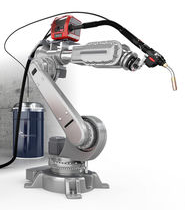
\includegraphics[width=6cm]{imagens/Fotos/Robo_de_proposito_geral.png}
                \caption{}
                \label{fig:robo_geral}
            \end{subfigure}
            \hfill
            \begin{subfigure}[b]{0.49\textwidth}
                \centering
                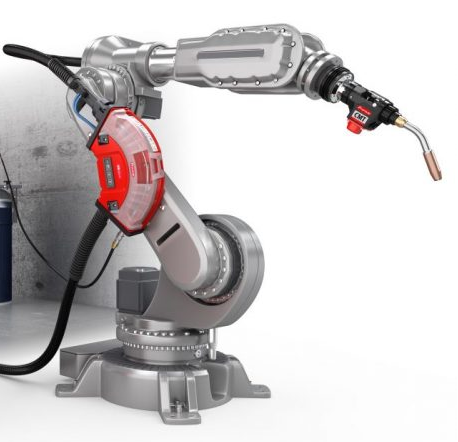
\includegraphics[width=7cm]{imagens/Fotos/Robo_dedicado.png}
                \caption{}
                \label{fig:robo_dedicado}
            \end{subfigure}
            \caption{Robô de propósito geral (a) e dedicado à soldagem (b)}
            \label{fig:tipos}
        \end{figure}
        
        Com relação às partes constituintes, um robô industrial é dividido em sua estrutura mecânica, na unidade controladora e no \ac{TP}. Podem integrar o sistema robótico diferentes ferramentas, dispositivos auxiliares, como trilhos para movimentação do robô, e dispositivos periféricos, como mesas móveis do tipo pórtico.  
        
        Os robôs industriais tradicionais possuem a unidade controladora uma arquitetura fechada de controle e geração de trajetória fornecida pelo fabricante. Esse tipo de solução segue o paradigma a qual deve ser priorizada a robustez e confiabilidade do funcionamento e da execução das tarefas, além de atender a certos requisitos normativos e legais que regem as indústrias. A controladora desses robôs é programada via uma linguagem dedicada, normalmente derivada de uma linguagem de programação de propósito geral acrescentada das funcionalidades necessárias aos robôs, como os comandos MOVE. Logo, cada fabricante de robô possui sua própria linguagem dedicada, os robôs ABB são programados na linguagem RAPID, os robôs Kuka em KRL, os robôs Comau em PDL2, etc. A linguagem PDL2 é derivada da linguagem PASCAL, por exemplo.
        
        Portanto, as controladoras fechadas buscam atender os requisitos de confiabilidade e também de simplicidade, demandando pouco conhecimento ou treinamento para operar ou programar um robô. No entanto, é perceptível que essa forma dificulta a realização de novas implementações e atividades de pesquisa com os robôs industriais. Ao mesmo tempo que estabelece, em certo ponto, uma dependência com os fabricantes e/ou com as empresas parceiras quando surge a necessidade de uma mudança ou expansão da célula de produção robotizada.
        
        Existem alguns fabricantes de robôs industriais, como a Comau, a Universal Robots, a Staubli e a Kuka, que possuem a opção de controladora aberta, isto é, controladoras que permitem programação utilizando linguagens de propósito geral, como C ou C++. A vantagem de usar esse tipo de linguagem, em comparação com o uso de uma linguagem dedicada à robótica, é que as possibilidades de uso são expandidas, por exemplo, é possível criar seu próprio gerador de trajetória, utilizar visão computacional para controlar a pose do robô, realizar um controle de força, substituir os controladores das juntas do robô, entre outras possibilidades. Isso vai mais ao encontro às novas demandas da Industria 4.0, bem como dos pesquisadores e desenvolvedores. Por exemplo, se surge a demanda por acrescentar uma malha de controle com visão computacional, poder-se-a integrar uma ou mais câmeras que tenham um bom custo, e não câmeras de um fornecedor específico, que geralmente apresentam custo mais elevado.  
        
        %DESVANTAGENS: Porque a maioria dos fabricantes de robôs industriais não possuem a opção de controladoras abertas?
        %(esta é uma das tais perguntas chave, no sentido de que vale a pena abordar e tentar responder)
        O paradigma de controladora aberta não atende todos os interesses das industrias, por exemplo, a industria demanda que a programação do equipamento seja facilmente aprendida por pessoas com baixa qualificação profissional e uma linguagem dedicada à robótica é concebida justamente com essa intenção, o que não é o caso do C e C++, já que, por serem de propósito geral, possuem muito mais funcionalidades do que apenas mover o robô por uma trajetória. Além disso, como comentado anteriormente, o paradigma da controladora fechada oferece mais robustez e confiabilidade de seu funcionamento e da execução das tarefas. 
        
        A Comau desenvolveu uma controladora aberta que é uma variante de sua controladora padrão. A abertura é realizada mediante a adição de um pequeno hardware de comunicação e um software ao PLC da controladora com objetivo de implementar a comunicação com um computador industrial fornecido pela fabricante. Neste computador são executado os programas desenvolvidos pelo usuário em C ou C++ com a possibilidade de controlar a posição, velocidade ou torque das juntas do robô, ao mesmo tempo que lê os dados sensoriais do robô. Dessa forma, a controladora aberta continua trabalhando da mesma forma que a controladora fechada, com a exceção de quando é ativada a modalidade aberta pela aplicação do usuário em sua linguagem dedicada, a PDL2, que está em execução na mesma. Quando isso acontece, a aplicação do usuário no computador industrial passa a comandar o robô. Logo, a solução da Comau pode ser considerada uma solução híbrida, permitindo ao usuário alternar entre usar a linguagem robótica para controlar o robô, ou usar a linguagem C/C++ para controlar o mesmo através da sua implementação.
        
        %Problema
        Apesar dessa solução inovadora, ela possui certas limitações, por exemplo, a linguagem de programação do desenvolvimento das aplicações é restrita à linguagem C ou C++, ao hardware fornecido pelo fabricante (o computador industrial) tanto em relação a potência computacional quanto à arquitetura do mesmo, ficando restrito também ao sistema operacional fornecido pelo fabricante.
        
        %Justificativa / Motivação
        Assim sendo, pareceu relevante a tentativa de se investigar se seria possível dar mais liberdade no desenvolvimento de aplicações para um robô industrial com controladora aberta, onde um terceiro dispositivo ficaria responsável por realizar todo o processamento necessário para a geração de trajetória e enviar essa referência de posição ao computador industrial fornecido pela fabricante do robô, que por sua vez repassaria a referência para a controladora do robô. Assim, tal computador industrial ficaria responsável por receber as referências e repassar para a controladora do robô.
        
        %Tema
        A proposta deste trabalho de conclusão de curso é desenvolver um arranjo cliente servidor para o computador industrial que possibilitará o desenvolvimento de aplicações em qualquer linguagem de programação, qualquer arquitetura e qualquer sistema operacional para um terceiro dispositivo que seja capaz de se conectar com o mesmo pelo protocolo \ac{TCPIP}, sendo o arranjo cliente servidor responsável apenas por ser uma ponte de comunicação entre a controladora do robô e o software rodando no terceiro dispositivo. Assim, dando mais liberdade aos desenvolvedores de aplicações para a Industria 4.0 e para os pesquisadores universitários, atendendo inclusive a demanda do Laboratório de Robótica do CEFET-MG, o qual possui uma controladora desse tipo, a C5G Open, disponível.
        
        %Colocar foto do robô e da controladora
        %\begin{figure}[!htb] 
        %    \centering
        %    \includegraphics[width=13cm]{Imagens/}%\columnwidth
        %    \small
        %    \centering
        %    \caption{Vista do sistema robótico no laboratório}
        %    \label{fig:introducao}
        %\end{figure}

	    %Hipótese
	    Parte-se da hipótese de que seja possível desenvolver um software que se comunique com a controladora do robô via protocolo fornecido pela fabricante ao mesmo tempo, porém em taxas diferentes, que se comunica com um software em um terceiro dispositivo via protocolo \ac{TCPIP}, sendo este terceiro dispositivo rodando um sistema operacional diferente, com uma arquitetura diferente e tal software em uma linguagem de programação diferente da exigida pela solução da fabricante. Assim, para viabilizar o teste dessa hipótese, realiza-se uma pesquisa de finalidade aplicada, objetivo exploratório, sob o método hipotético-dedutivo, com abordagem quantitativa, realizada com procedimentos experimentais. %Metodologia
        
    \section{Objetivos} %Objetivo geral     %Objetivos Específicos
        O objetivo geral do trabalho é desenvolver um software com arranjo do tipo cliente servidor, que estenda a liberdade que a solução de controladora aberta que a fabricante proporciona aos programadores de robôs industriais.
		
		\subsection{Objetivos específicos}
		    Para atingir o objetivo geral, é necessário desenvolver:
            \begin{itemize}
                \item Um protocolo de comunicação \ac{TCPIP} para enviar e receber variáveis referentes aos ângulos de juntas do robô.
                \item Uma função que salve na memória os ângulos de referência das juntas do robô oriundo do software no terceiro dispositivo, e que enviar os dados sensoriais armazenados na memória para tal software.
                \item Uma função use a solução da fabricante para ler dados sensoriais os salvando na memória e enviar referências das juntas do robô armazenadas na memória.
                \item E resolver o problema gerado pelo assincronismo da comunicação entre arranjo e controladora com o arranjo e o software no terceiro dispositivo.
            \end{itemize}
            
	\section{Organização do texto}  %Previa dos capítulos        %Hipótese        %Previa conclusão
	    
	    O Capítulo \ref{chp:Fundamentos} apresenta a revisão teórica do tema e assuntos tratados.  %apresenta o referencial teórico do tema e a referência bibliográfica dos assuntos tratados.
	    
	    O Capítulo \ref{chp:Desenvolvimento} apresenta o desenvolvimento do software arranjo cliente servidor e de um software cliente exemplo para realizar os testes e coletar os resultados experimentais.
	    
	    Já o Capítulo \ref{chp:Resultados} apresenta os resultados experimentais e discute a consequência deles.
	    
	    Ao final deste trabalho conclui-se no Capítulo \ref{chp:Conclusão} que o objetivo de estender a liberdade que a solução da fabricante proporciona aos programadores de robôs industriais foi atingido.

    \chapter{Fundamentação}
    \label{chp:Fundamentos}

	\section{Controladora Robótica Aberta}
	
        Algumas tentativas feitas pela academia foram relatadas na literatura no sentido de abrir a estrutura de controle de alguns robôs industriais~\cite{ROBERTI:2010}. Recentemente, alguns fabricantes de robôs perceberam essa demanda por parte das instituições de ensino e pesquisa e, de forma semelhante ao que vem acontecendo com os softwares de código aberto do \textit{ROS} (Sistema Operacional Robótico, em tradução livre), passaram a oferecer a opção de abertura do sistema de controle de robôs~\cite{KUBUS:2010}, isto é, uma controladora aberta. 
        
        Uma opção para atender essa demanda foi desenvolvida pelo fabricante de robôs industriais \textit{Comau}, adicionando uma arquitetura complementar à controladora de seus robôs, a \textit{Comau C5G}. Essa extensão, denominada \textit{Comau C5G Open Controller}, é feita através da conexão da controladora a um computador industrial externo, denominado \ac{LPC}, por intermédio de uma conexão \textit{Ethernet PowerLink}, como é mostrado na Figura~\ref{controladora2}~\cite{ANTONELLI:2010}.
        
        A Figura~\ref{controladora} permite a visualização da solução fornecida pelo fabricante, sendo que, a conexão \textit{Ethernet} \ac{TCPIP} precisa ser intermediada por um modem, roteador ou \textit{switch} não fornecido nessa extensão.
        
        \begin{figure}[ht]
            \centering
            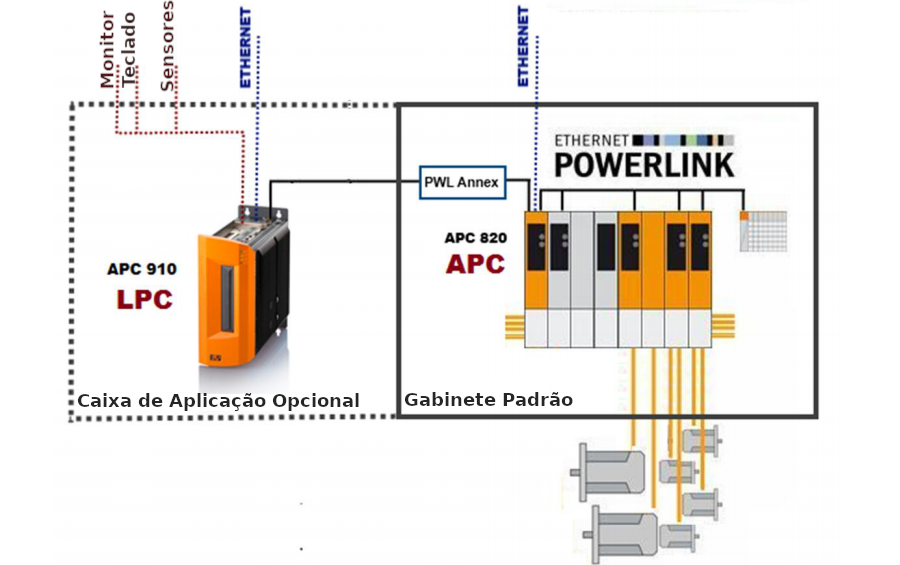
\includegraphics[width=\columnwidth]{imagens/Conexoes/controladora2.png}
            \small 
            \centering 
            \caption{Visão geral sobre o hardware do sistema C5G-Open}
            Adaptado de~\cite{Ferrara:2013}
            \label{controladora2}
        \end{figure}
        
        Assim, é possibilitado à controladora do robô industrial enviar dados sensoriais e receber referências de um software a ser programado pelo usuário, a taxas de até 1 pacote a cada \SI{0,4}{\milli\second} (1 pacote contém todas as leituras de sensores do robô). Isso possibilita a criação de softwares que implementem malhas de controle adicionais como: controle de força, visão computacional, entre outros.~\cite{Ferrara:2013}
        
        \begin{figure}[ht]
            \centering
            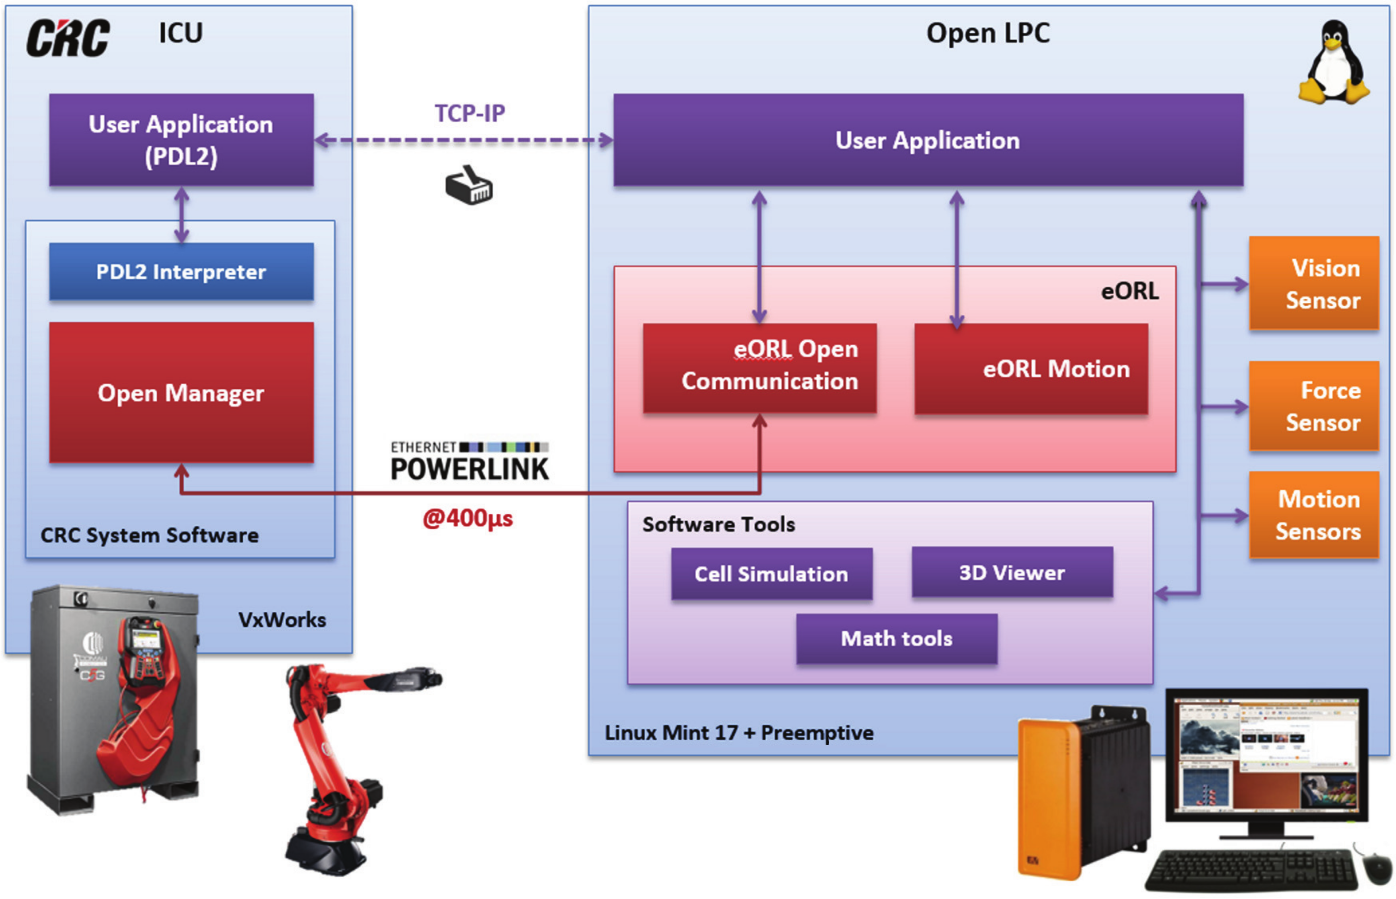
\includegraphics[width=\columnwidth]{imagens/Conexoes/controladora.png}
            \small 
            \centering 
            \caption{Visão geral do software do sistema C5G-Open}
            Fonte:~\cite{Open:Manual}
            \label{controladora}
        \end{figure} 
        
        Entretanto, existem algumas limitações, por exemplo: o software (\textit{User Application} na Figura \ref{controladora}) que implementa essa malha de controle adicional precisa ser compilado e executado nesse computador industrial externo, rodando o sistema operacional \textit{Linux Mint 17} compilado para arquitetura x86, conectado à controladora por um cabo de rede especial chamado \textit{Ethernet PowerLink} (visto na Figura \ref{controladora}). Ele precisa ser programado em C/C++ e utilizar a biblioteca proprietária de código fechado desenvolvida pela \textit{Comau} chamada \ac{eORL}, para controlar a comunicação.%Citar manual c5gopen
        
        Além disso, uma utilização inadequada por um usuário que deixe a conexão com o \ac{LPC} habilitada do lado da controladora e que não tenha a adequada resposta do lado do \ac{LPC}, por exemplo, poderá produzir um erro de comunicação que acabará sendo armazenado em seus registros e impedirá a liberação dos \textit{drivers} da controladora pelo seu módulo de gerenciamento de segurança, chamado C5G-SDM (Módulo de Distribuição e Segurança, em português)~\cite{C5G:Manual}, como já aconteceu na controladora do Laboratório de Robótica do CEFET-MG uma vez.
        
        Por fim, nem todos os programas necessários para o desenvolvimento de aplicações podem ser instalados no \ac{LPC}, como é o caso do \textit{ROS}, devido ao fato que os drivers do Powerlink Card precisam de uma versão mais antiga do Sistema Operacional Ubuntu (ou derivados dele, como Linux Mint) para funcionar~\cite{Bisson:2014}. Atualmente é executado no \ac{LPC} a versão 17 do Linux Mint, que é baseado na versão \ac{LTS} de 2014 do Ubuntu. Então, todos os programas e versões de bibliotecas do sistema operacional são versões ultrapassadas e, geralmente, não oferece suporte à instalação das novas versões dos mesmos, como é o caso do \textit{ROS 2}, que é a mais nova versão do \textit{ROS}.
        
        Para utilizar o sistema \textit{Open} é necessário a instalação da biblioteca \ac{eORL} no \ac{LPC} na mesma versão da \ac{eORL} da controladora~\cite{Open:Manual}. Além disso, é necessário habilitar o modo Open nos eixos desejados através da controladora antes de utilizar a modalidade. Para isso, é usado o programa \textit{Crcopen} disponível na controladora, conforme indicado na Figura~\ref{habilitar-open}.
        
        \begin{figure}[ht]
            \centering
            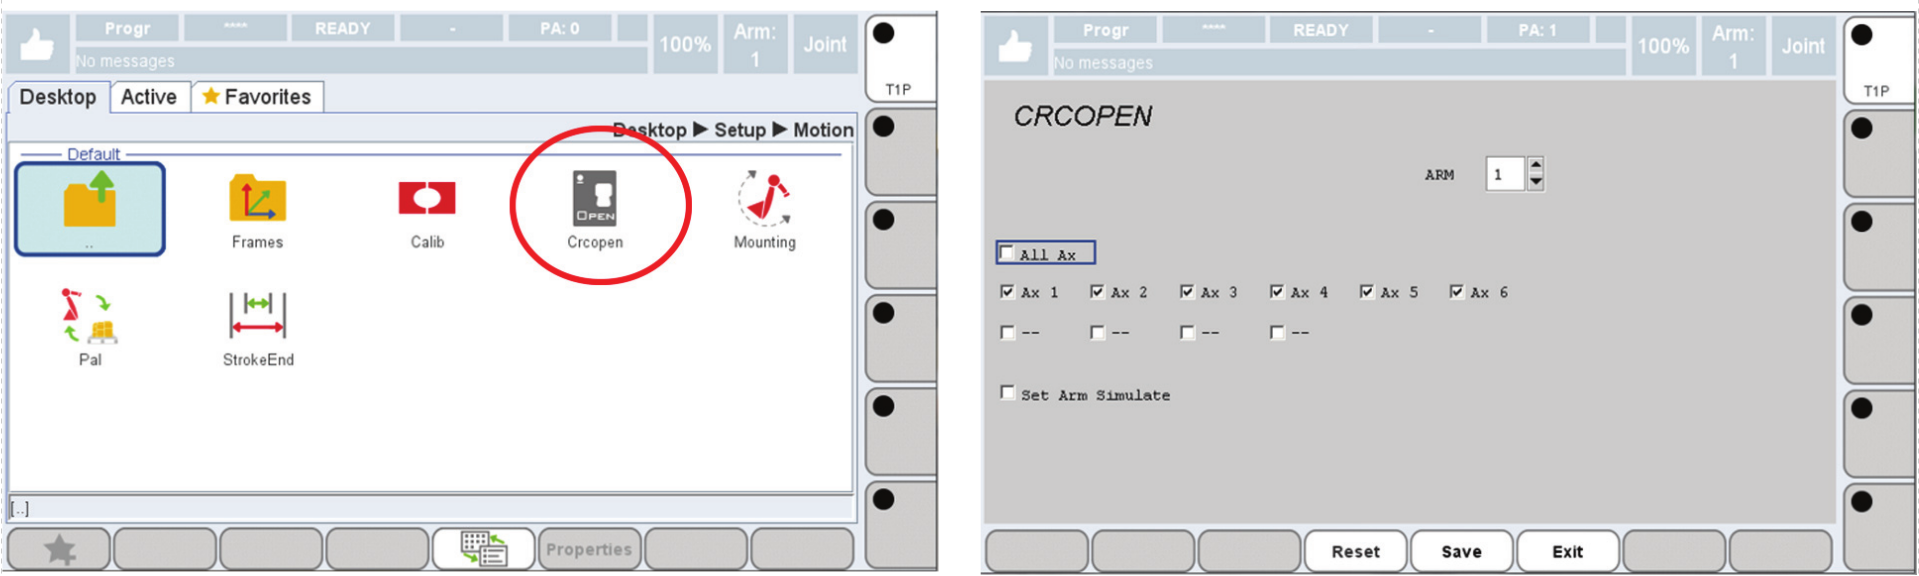
\includegraphics[width=\columnwidth]{imagens/Softwares/habilitar-open.png}
            \small 
            \centering 
            \caption{Procedimento para habilitar o modo Open dos eixos do robô~\cite{Open:Manual}}
            \label{habilitar-open}
        \end{figure}
        
    \section{Modo de Simulação}
        
        %Estou escrevendo essa subseção agora, depois você revisa
        A fabricante da controladora desenvolveu um modo de simulação para realizar testes com segurança das tarefas a serem preparadas no sistema Open. Este modo de simulação envia um comando para os controladores dos motores não atuarem nos motores e não lerem os sensores. Ao invés disso, ele irá usar a resposta esperada dos motores para estimar os valores dos respectivos sensores. Desta forma o robô permanece seguro sem se mover até que seja reiniciado o robô sem o modo de simulação.
        
        \begin{figure}[!htb] 
            \centering
            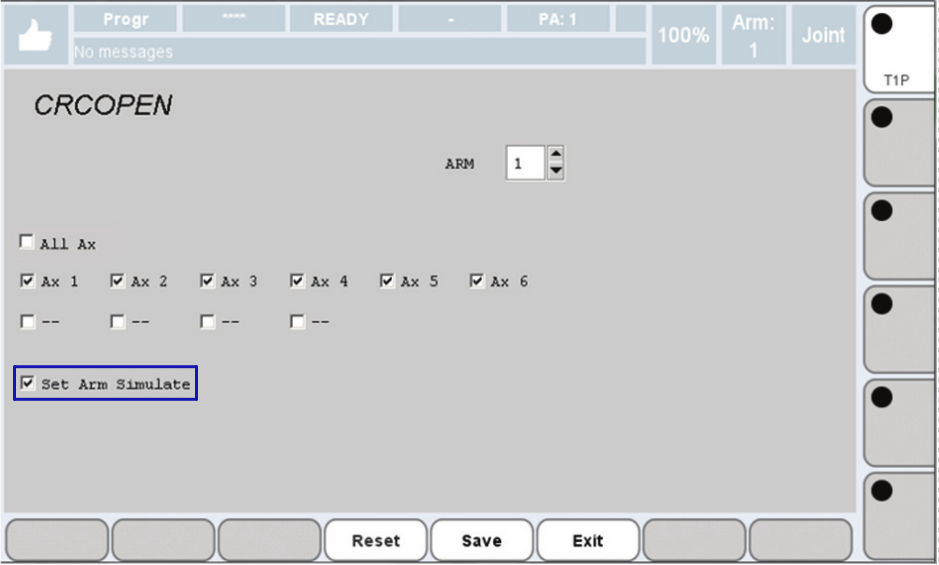
\includegraphics[width=10cm]{imagens/Softwares/habilitar-simu.png}%\columnwidth
            \small
            \centering
            \caption{Ativando o modo de simulação. Adaptado de~\cite{Open:Manual}}
            \label{fig:habilitar_simu}
        \end{figure}
        
        Existem três maneiras de visualizar os ângulos das juntas do robô no modo simulação: através da janela do programa MOTION no \ac{TP}; ou através da aplicação a ser desenvolvida pelo usuário do sistema Open (nesse caso, os pacotes de dados sensoriais que o \ac{LPC} irá receber na verdade conterão as estimações dos ângulos das juntas); ou através de um software chamado \textit{Comau Visual3D}, desenvolvido pela fabricante com a finalidade de visualizar virtualmente o robô, simulado ou não.
        
        O \textit{Visual3D} comunica-se diretamente com a controladora através da rede Ethernet, a qual a controladora está conectada, e possui o armazenado na memória dos modelos 3D de vários robôs da fabricante. Quando ele se comunica com a controladora pela primeira vez, ele recebe a informação de qual robô está conectado à controladora. Então, passa a receber continuamente os valores angulares de cada junta do robô, usando esses dados para realizar, em tempo real, uma renderização 3D do modelo do robô na \ac{POSE} determinada por esses valores. Na Figura~\ref{fig:visual} são mostrados exemplos de visualização fornecidos pelo do programa \textit{Visual3D} exibindo o robô virtual.
        
        \begin{figure}[h]
            \centering
            \begin{subfigure}[b]{0.4\textwidth}
                \centering
                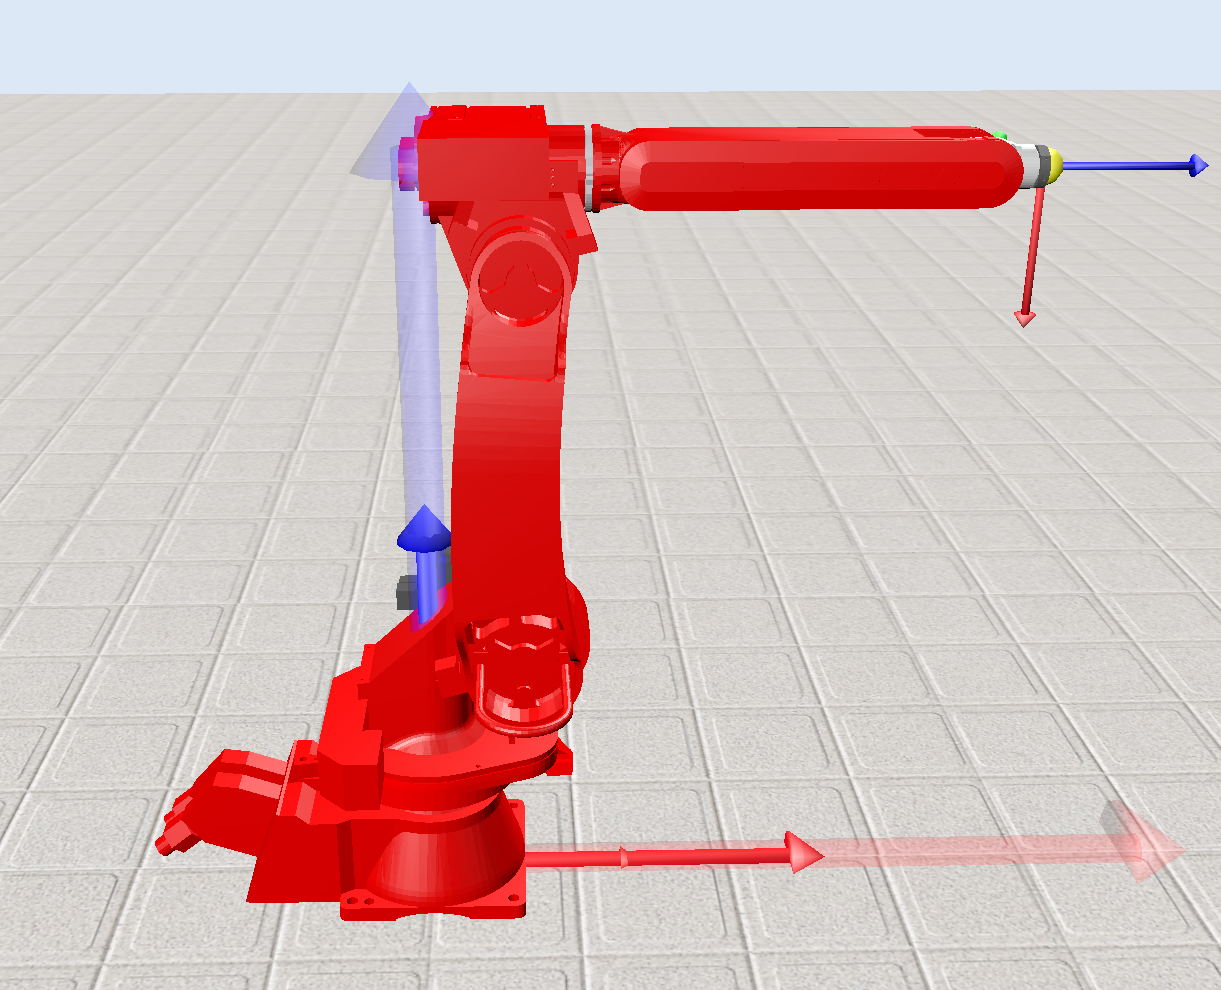
\includegraphics[width=60mm]{imagens/Softwares/visual3d-a.png}
                \caption{}
                \label{fig:visuala}
            \end{subfigure}
            \hfill
            \begin{subfigure}[b]{0.4\textwidth}
                \centering
                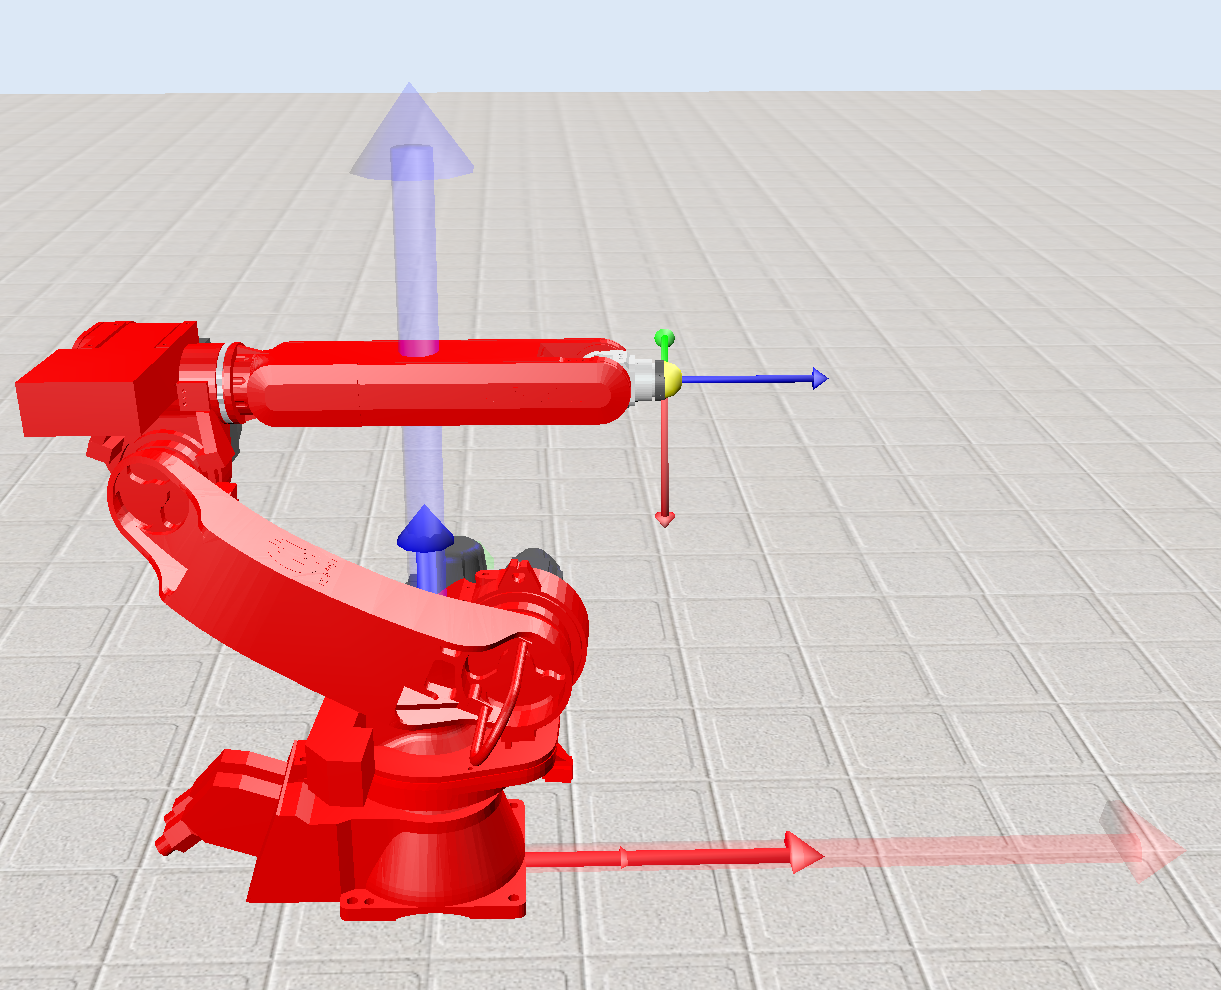
\includegraphics[width=60mm]{imagens/Softwares/visual3d-b.png}
                \caption{}
                \label{fig:visualb}
            \end{subfigure}
            \caption{Modelo 3D do robô no software Visual3D em duas \ac{POSE}'s distintas}
            \label{fig:visual}
        \end{figure}
        
        Como este programa apenas oferece uma visualização gráfica do robô para o usuário, ele não é necessário para utilizar o sistema Open ou o modo de simulação. No entanto, o \textit{Visual3D} é de grande auxílio nos testes de programas desenvolvidos para o sistema Open em modo de simulação, pois permite identificar mais facilmente se o teste simulado está ocorrendo conforme esperado, do que analisando os valores dos ângulos ou da pose do robô no \ac{TP}.
    
    \section{Ponteiro Inteligente}

        Um ponteiro inteligente é um tipo de dado implementado na linguagem de programação \textit{C++} partir da revisão \textit{C++11}. Esse tipo de dado fornece recursos adicionais aos ponteiros, como gerenciamento automático de memória. No caso, eles controlam automaticamente a memória para a qual apontam e deletam automaticamente o objeto apontado após a utilização, por exemplo, porque o proprietário é uma variável local, e a execução sai do escopo da variável.~\cite{cppreference}
        
        O Ponteiro Inteligente utilizando no desenvolvimento deste trabalho é o shared\_ptr. Ele é um ponteiro compartilhado e tem a característica de nenhum shared\_ptr específico possuir algum objeto. Todos os shared\_ptr que apontam para o mesmo objeto colaboram para garantir sua existência e quando todos deixam de apontar para tal objeto ele é destruído automaticamente.~\cite{meyers2015} 
        
    \chapter{Desenvolvimento}%
    \label{chp:Desenvolvimento}
	
	\section{O OpenServer}
	
    	Visando oferecer mais liberdade e flexibilidade para o usuário, no que diz respeito à programação da malha de controle adicional e ao dispositivo que irá executá-la, foi desenvolvido um programa chamado OpenServer, isto é, o servidor do sistema Open. Este, tem também o objetivo de trazer mais segurança para a controladora do robô do laboratório do CEFET-MG em Divinópolis durante a execução de malhas de controle experimentais. 
    	
    	O OpenServer é executado no LPC e utiliza a biblioteca \ac{eORL} para intermediar a comunicação entre a controladora robô e o LPC, ou seja, utiliza a estrutura do sistema Open fornecida pela fabricante. Ele oferece uma \textit{API} (Interface de Programação de Aplicativo, em tradução livre) baseada em rede \ac{TCPIP} para se comunicar com um programa cliente em um terceiro dispositivo. Este programa cliente tem o papel de enviar as referências das juntas do robô para o OpenSever, que por sua vez tem que repassar estas referências para a controladora do robô. Ao mesmo tempo, o OpenSever tem o papel de receber da controladora os dados sensoriais do robô (posição angular das juntas, por exemplo) e repassar para o programa cliente. Como a comunicação entre controladora e o LPC pode ocorrer a uma taxa diferente da comunicação do LPC com o terceiro dispositivo, o OpenServer tem que conseguir realizar a comunicação de forma assíncrona. 
    	
    	O objetivo é que o programa cliente possa ser escrito em qualquer linguagem de programação que suporte o protocolo \ac{TCPIP} e que possa rodar em qualquer sistema operacional que tenha suporte ao mesmo. E que o dispositivo no qual o programa cliente esteja rodando possa ser de qualquer arquitetura de processador, desta forma, permitindo que até dispositivos móveis como \textit{smartphones} que utilizem a \textit{API} do OpenServer.
        
        Acredita-se que essa abordagem possa reduzir riscos ao equipamento por erro ou imperícia ao ser programada uma malha de controle usando recursos do sistema \textit{Open} fornecidos pelo fabricante. Pois o OpenServer pode ser programado para continuar se comunicando com a controladora, mesmo que a conexão com o programa cliente seja perdida ocasionada por um fechamento inesperado do programa cliente ou um travamento, enquanto que, se este programa estivesse sendo executado no LPC, a comunicação com a controladora seria encerrada bruscamente. Além disso, o OpenServer é capaz de oferecer uma alternativa de \textit{API} mais simples de ser aprendida e utilizada.
	
        A estrutura padrão do sistema fornecida pela empresa fabricante é detalhada na Figura~\ref{conexoes-padrao}, onde: (1) é a conexão elétrica entre Controladora e Manipulador Robótico; (2) representa a conexão \textit{PowerLink} entre \ac{LPC} e controladora; (3) é a conexão entre roteador e controladora; e (4) conexão entre roteador e o \ac{LPC}.
    
        \begin{figure}[ht]
            \centering
            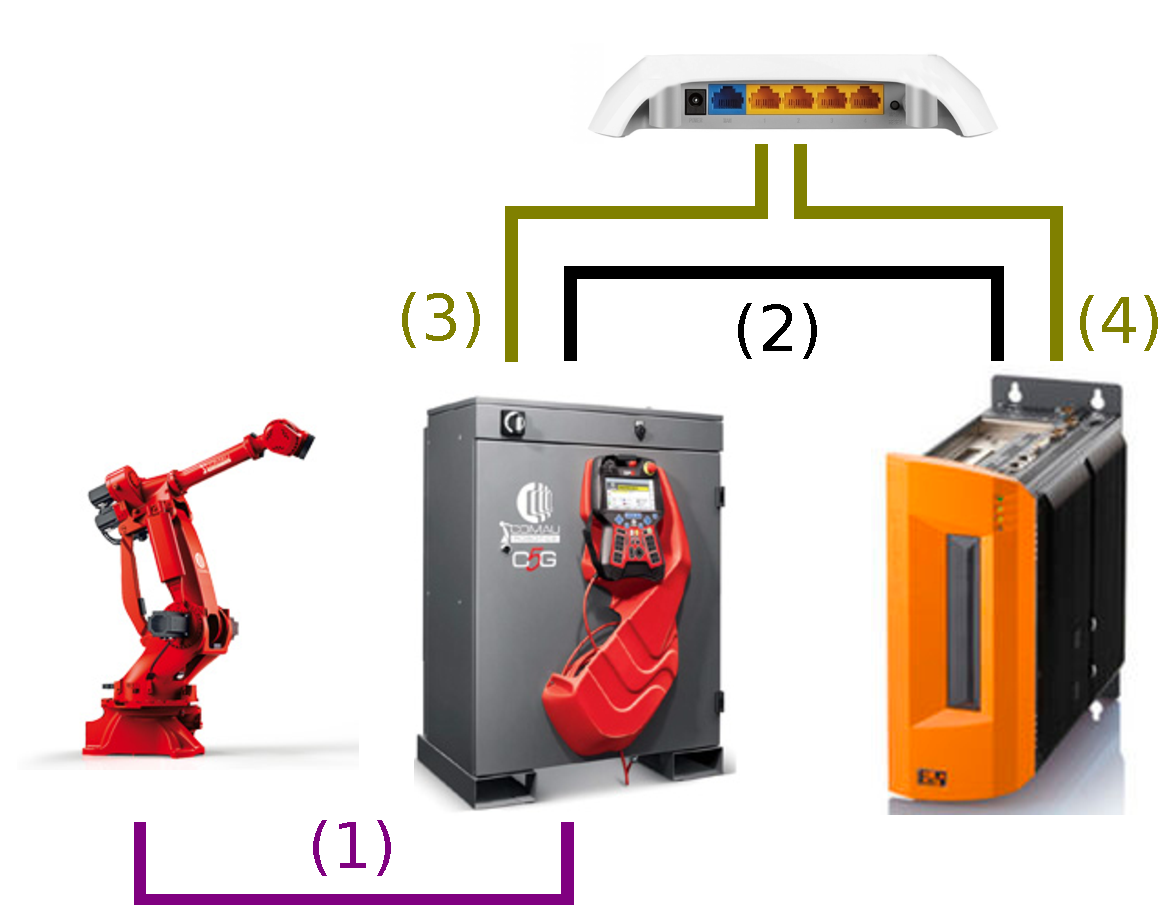
\includegraphics[width=10cm]{imagens/Conexoes/conexoes-padrao.eps}
            \small 
            \centering 
            \caption{Estrutura padrão do sistema C5G Open}
            \label{conexoes-padrao}
        \end{figure}
          
        Como dito anteriormente, o OpenServer foi desenvolvido para utilizar-se a estrutura padrão do sistema fornecida pela empresa fabricante. Logo, foi programado dentro das limitações da plataforma, ou seja, na linguagem C++ usando a biblioteca \ac{eORL} do fabricante do robô, sendo usada a conexão \textit{Ethernet PowerLink} do LPC para fazer a comunicação com a controladora do robô e sendo compilado para o sistema operacional baseado em Linux com arquitetura x86. Além disso, ele usa a rede \textit{Ethernet} convencional do LPC e bibliotecas padrão em C++ disponíveis para o sistema operacional \textit{Linux Mint} para realizar a comunicação via protocolo \ac{TCPIP}. A estrutura desenvolvida para execução do OpenServer passa então a ser conforme é mostrado na Figura~\ref{conexoes-openserver}, onde: (5) representa a conexão entre o roteador e o dispositivo externo, que pode ser feita através de cabeamento ou conexão sem fio; e (6) é a conexão entre roteador e rede institucional.
        
        \begin{figure}[ht]
            \centering
            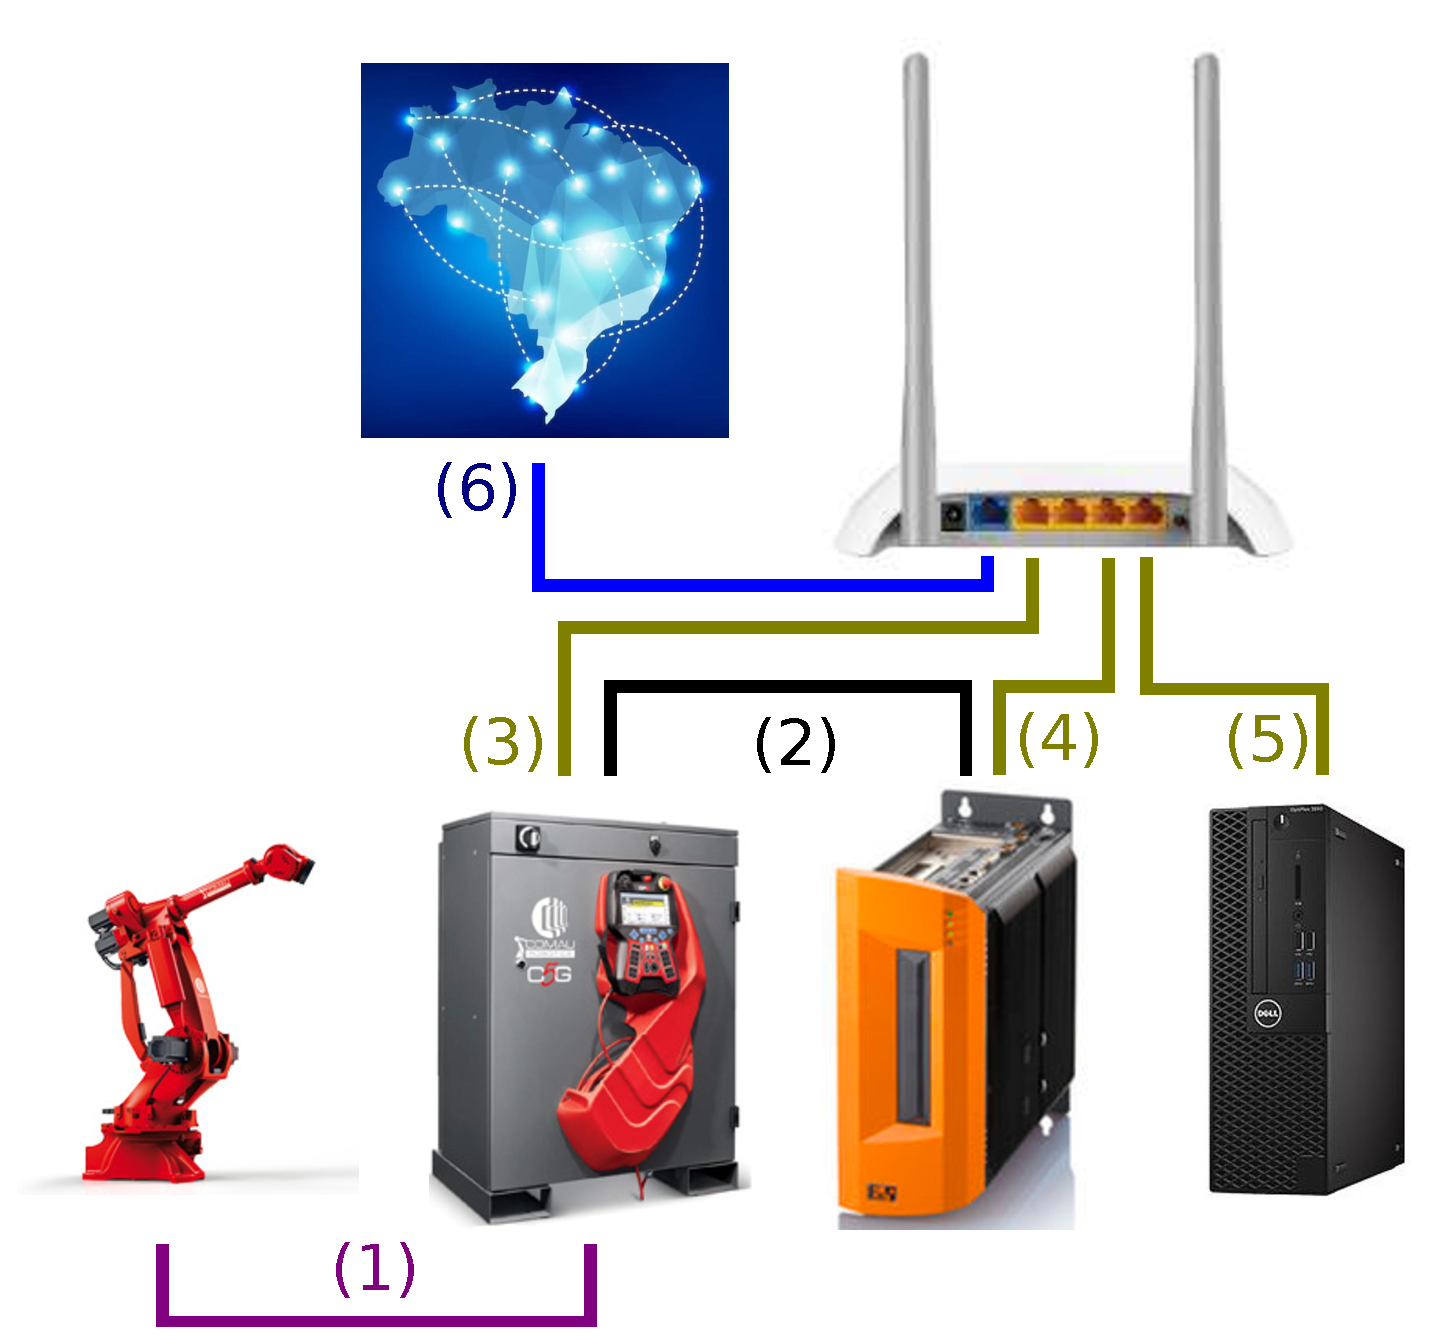
\includegraphics[width=10cm]{imagens/Conexoes/conexoes-openserver.eps}
            \small 
            \centering 
            \caption{Estrutura desenvolvida para execução do OpenServer}
            
            \label{conexoes-openserver}
        \end{figure}
        
        A rede institucional do CEFET-MG oferece acesso à internet. No entanto, as portas do roteador são bloqueadas para acesso externo. Dessa forma, é criada uma rede interna segura onde os programas se comunicarão. Por esta razão, não foram implementadas soluções de criptografia de dados, bem como de autenticação. Isso ocorreu também pelo motivo de ser um ambiente acadêmico, controlado e sem trafego de dados sensíveis. A estrutura real do sistema pode ser visto na Figura~\ref{lab1}. Estão disponíveis também dois computadores conectados à rede interna, que podem ser vistos na Figura~\ref{lab2}, para a execução de programas clientes.
        
        \begin{figure}[ht]
            \centering
            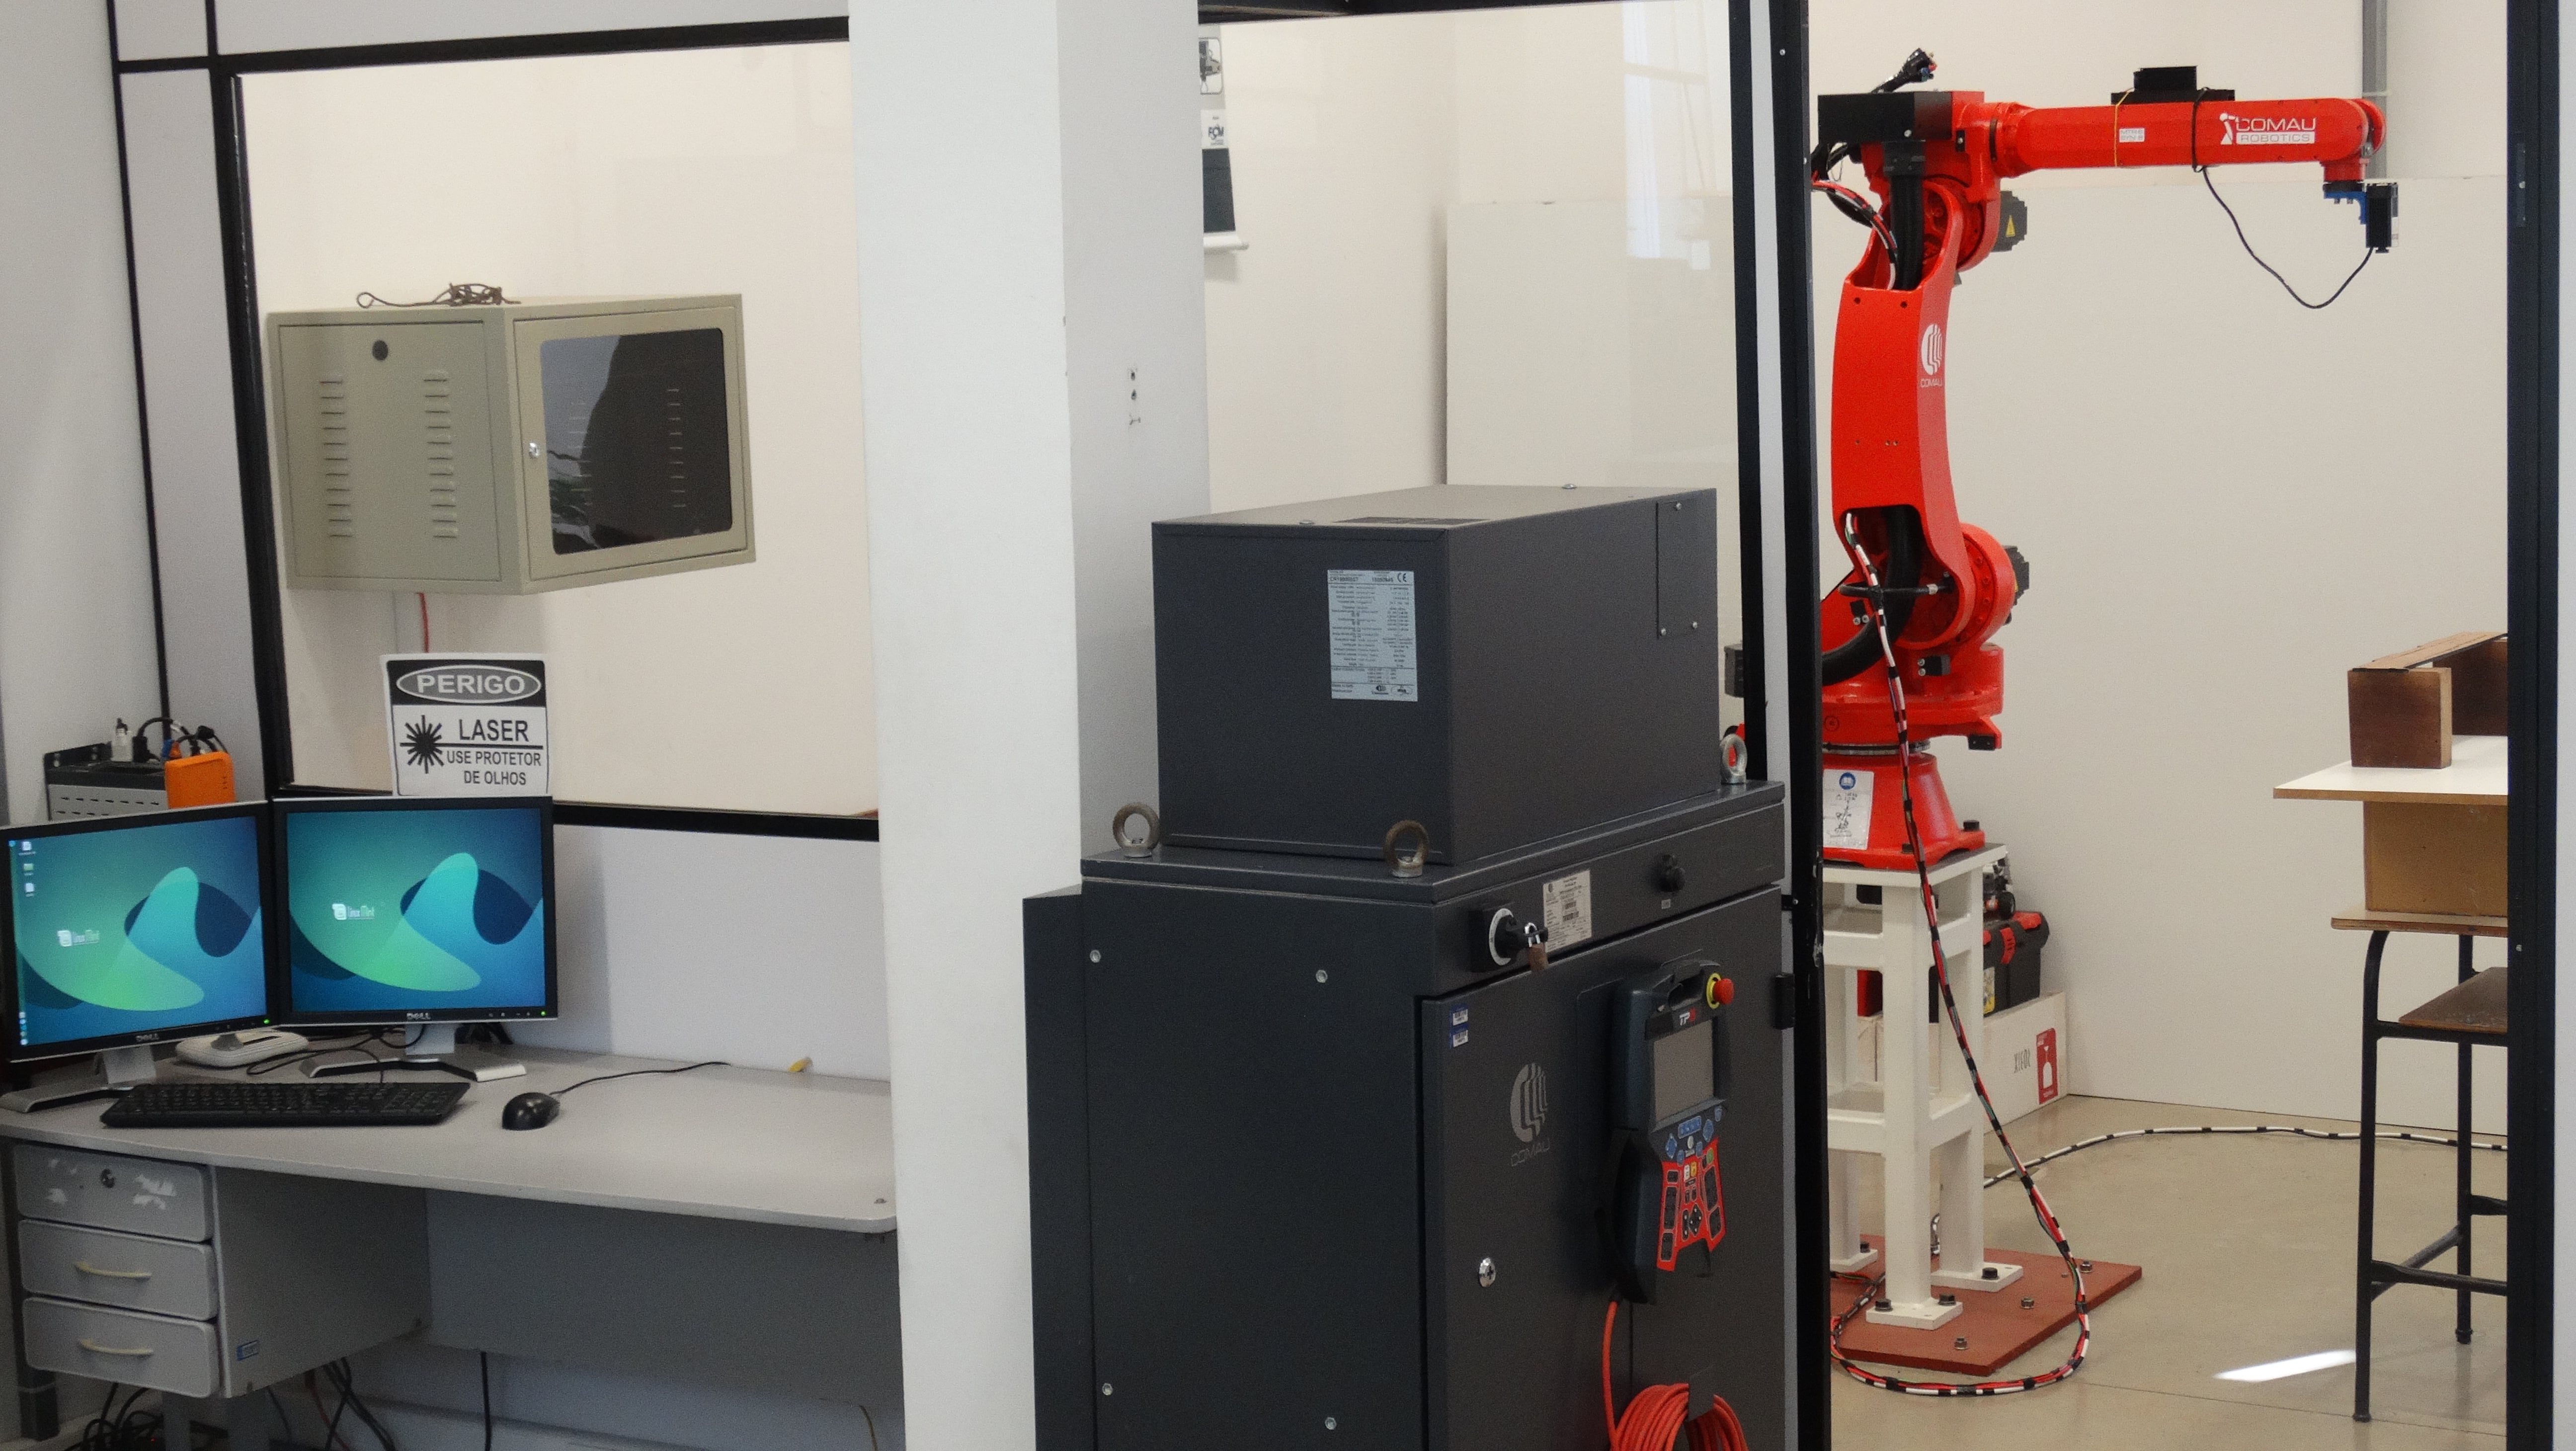
\includegraphics[width=\columnwidth]{imagens/Fotos/estrutura-lab-1.JPG}
            \small 
            \centering 
            \caption{Estrutura do laboratório: robô, controladora e \ac{LPC}}
            \label{lab1}
        \end{figure}
        
        \begin{figure}[ht]
            \centering
            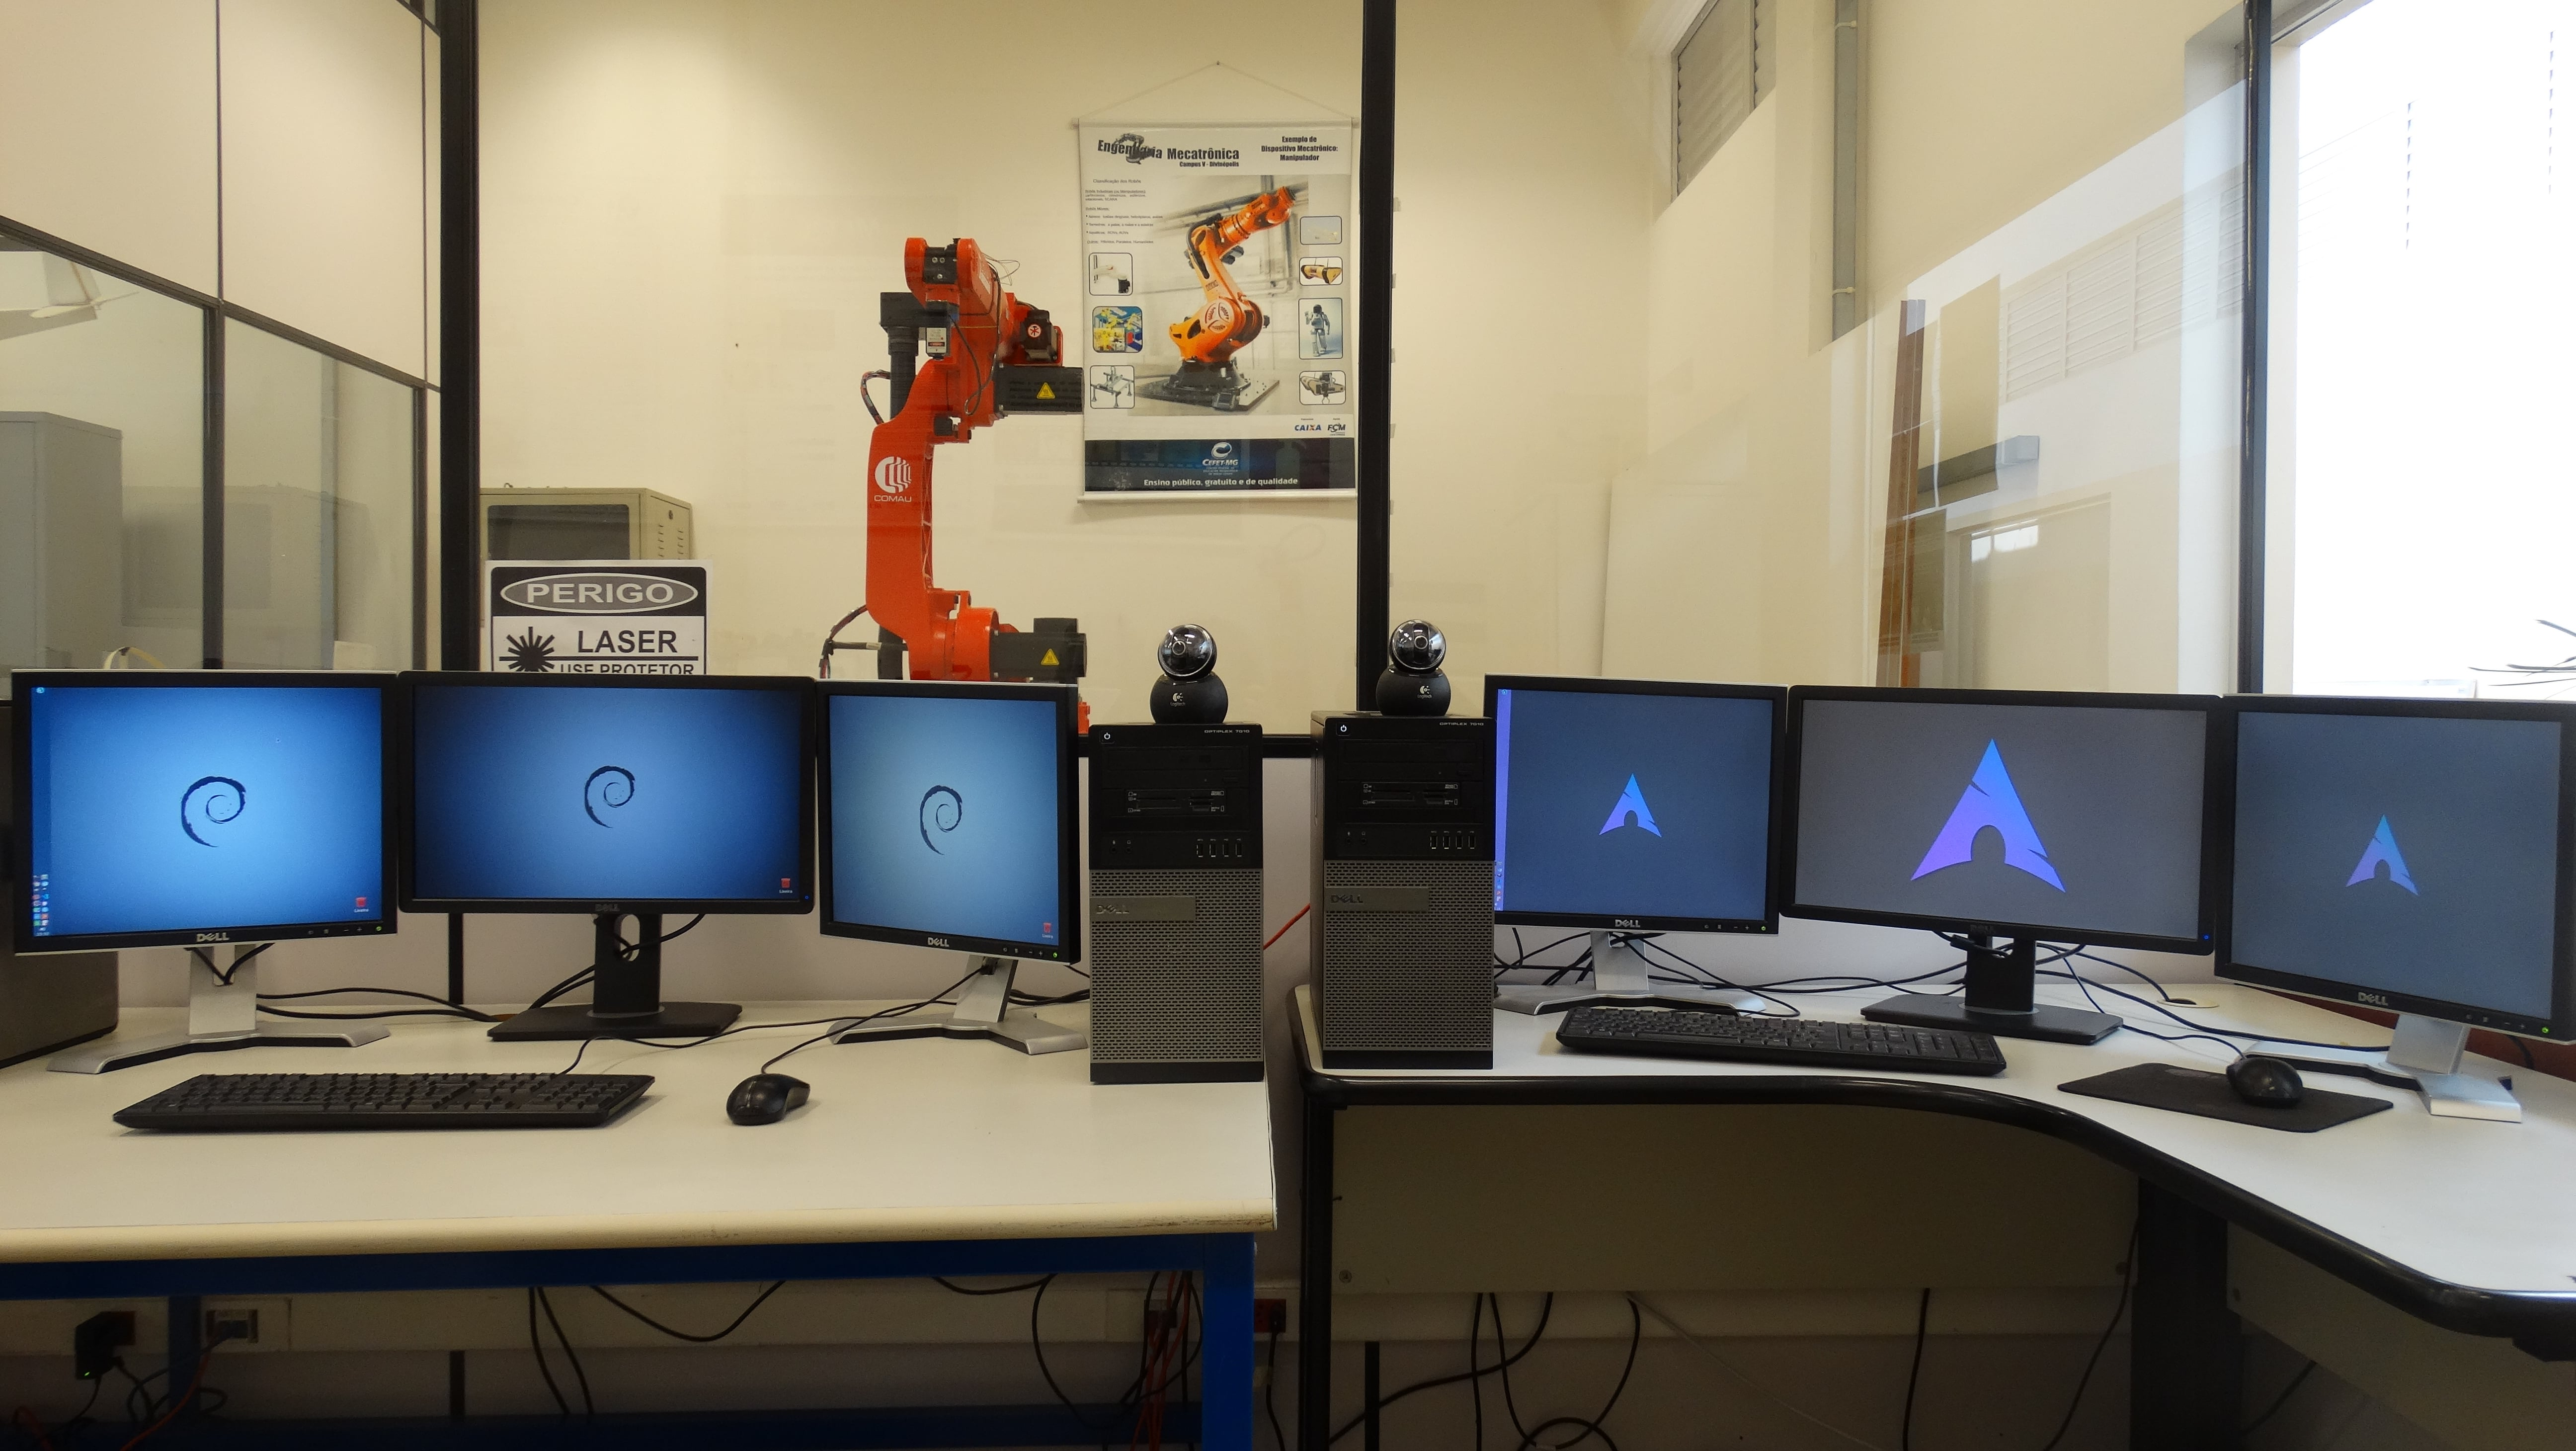
\includegraphics[width=\columnwidth]{imagens/Fotos/estrutura-lab-2.JPG}
            \small 
            \centering 
            \caption{Estrutura do laboratório: computadores onde serão executados os programas clientes}
            \label{lab2}
        \end{figure}
        
        O desenvolvimento desta abordagem torna mais segura a utilização do sistema Open em um ambiente de ensino e pesquisa, pois o único programa que precisará ser executado no \ac{LPC} passa a ser o \textit{OpenSever} em uma versão estável. Já no dispositivo externo serão executados os programas experimentais ou em desenvolvimento, os quais podem travar durante a execução, por exemplo, entre outros acontecimentos que podem gerar uma falha de comunicação. Em caso de algo assim acontecer, o \textit{OpenSever} continua sendo executado no \ac{LPC} e comunicando com a controladora do robô, enviando a última referência armazenada na memória, até que o programa cliente se reconecte ou o OpenServer receba o comando de desligar a comunicação. Dessa forma, o risco de se interromper bruscamente a comunicação com a controladora é evitado.
        
        Além disso, o \textit{OpenSever} expõe apenas um subconjunto das funcionalidades e configurações da \ac{eORL}, simplificando a utilização e reduzindo a quantidade de erros possíveis.
    
        \subsection{Funcionamento}
        
            Foi implementado um modo \textit{DEBUG}, a ser ativado antes do processo de compilação que imprime no terminal qual função foi executada, o comando vindo do programa cliente e a resposta enviada, conforme pode ser visto nas Figuras~\ref{openserver-wait}, \ref{openserver-ok}~e~\ref{openserver-send}. Quando o modo \textit{DEBUG} não está ativado, apenas a biblioteca \ac{eORL} imprime textos no terminal, por exemplo, a tela de boas vindas, mensagens de erro, entre outros.
            
            Quando o programa é executado, ele tenta se conectar com a controladora usando a biblioteca \ac{eORL} através da conexão \textit{Ethernet Powerlink}. Quando a conexão é bem sucedida o programa entra em modo \textit{Listen}, ou seja, fica esperando um cliente se conectar ao \textit{soket} através da rede \ac{TCPIP} via \textit{Ethernet} convencional, conforme pode ser visto na Figura~\ref{openserver-wait}.
            
            \begin{figure}[ht]
                \centering
                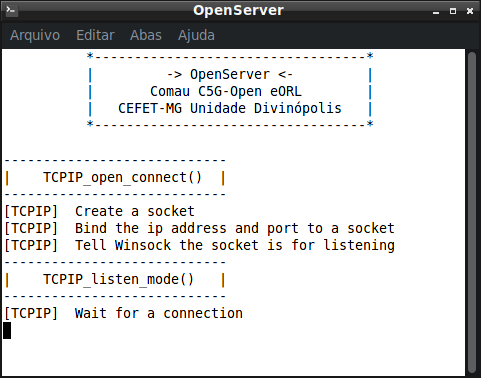
\includegraphics[width=10cm]{imagens/Softwares/openserver-wait_.png}
                \small 
                \centering 
                \caption{OpenServer esperando a conexão de um programa cliente}
                \label{openserver-wait}
            \end{figure}
            
            Quando um cliente se conecta ao servidor é realizada uma troca de pacotes para verificar a integridade da conexão. Caso essa verificação seja bem sucedida o servidor fica esperando o recebimento de instruções do cliente, conforme pode ser visto na Figura~\ref{openserver-ok}. O servidor só atua mediante os comandos do cliente.
            
            \begin{figure}[ht]
                \centering
                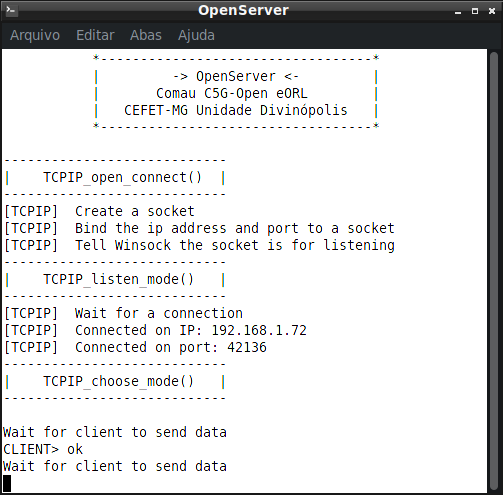
\includegraphics[width=10cm]{imagens/Softwares/openserver-ok_.png}
                \small 
                \centering 
                \caption{OpenServer esperando a instrução do programa cliente conectado}
                \label{openserver-ok}
            \end{figure}
            
            O primeiro caractere recebido pelo servidor informa qual procedimento ele deve seguir. No caso, a instrução `p' é atualmente a instrução padrão, ela está configurada para logo após virem os valores de referência das juntas do robô (truncado em 5 casas decimais, mas, sem uso da vírgula para representar as casas decimais) concatenados na forma de \textit{strings}, como pode ser visto na Figura~\ref{openserver-send}. Ao receber essa instrução, imediatamente o servidor atualiza as variáveis de referência das juntas do robô na memória do programa, que através da \ac{eORL} são enviadas para a controladora. Em seguida, também na forma concatenada sem uso de virgula, o servidor envia a resposta ao programa cliente com a leitura mais recente dos sensores das juntas do robô armazenada na memória do servidor, as quais foram recebidas da controladora.
            
            \begin{figure}[ht]
                \centering
                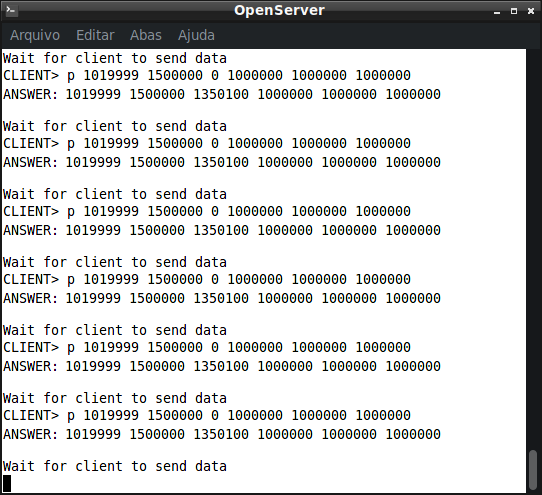
\includegraphics[width=10cm]{imagens/Softwares/openserver-send_.png}
                \small 
                \centering 
                \caption{OpenServer executando a instrução do programa cliente e respondendo com a leitura dos sensores}
                \label{openserver-send}
            \end{figure}
            
            Esta forma de transmitir os dados (\textit{strings} concatenadas) foi desenvolvida com a intenção de ser uma construção simples de ser implementada em outras linguagens de programação.
            
            Para ilustrar o funcionamento em simultâneo do OpenServer, programa cliente e controladora, bem como a comunicação entre eles, foi desenvolvido um fluxograma contendo o funcionamento desta estrutura. O mesmo pode ser visualizado na Figura~\ref{fig:fluxograma}, onde as setas na cor preta mostram o fluxo de funções do programa; as setas na cor ciano indicam a comunicação \textit{Ethernet} entre o dispositivo do cliente e o \ac{LPC}; e as setas na cor magenta indicam a comunicação do \textit{OpenServer} com a controladora do robô.
            
            \begin{figure}[ht]
                \centering
                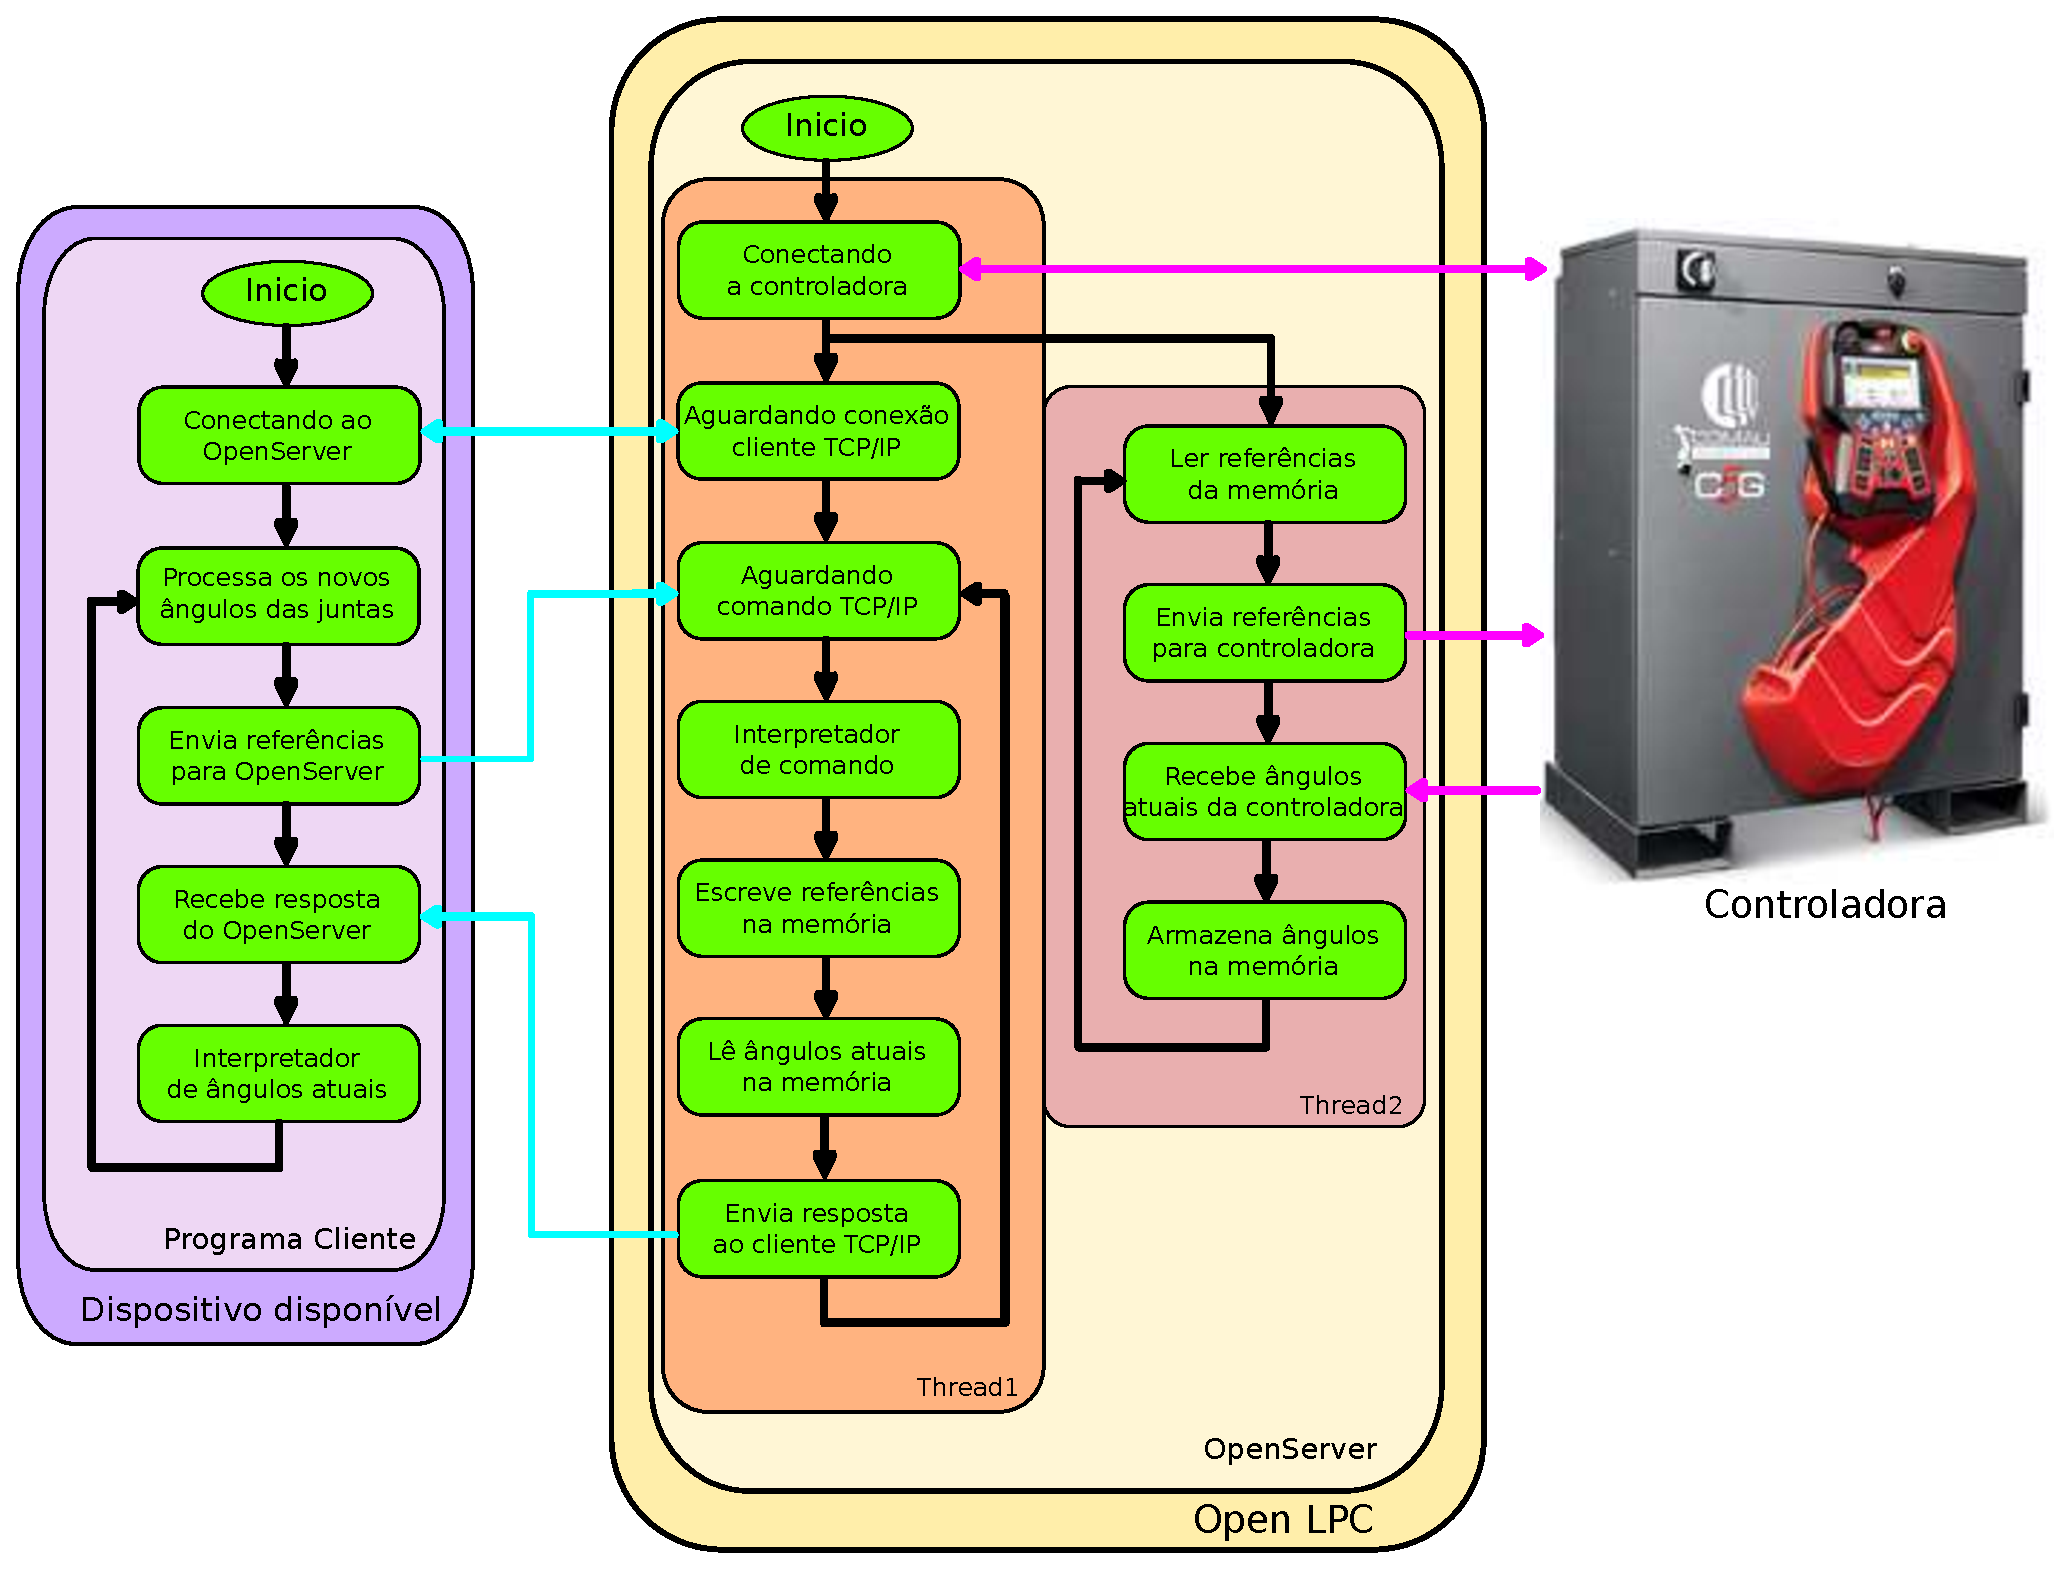
\includegraphics[width=\columnwidth]{imagens/Softwares/infografico.eps}
                \small 
                \centering 
                \caption{Fluxograma do funcionamento e comunicação do OpenServer, programa cliente e controladora.}
                \label{fig:fluxograma}
            \end{figure}
            
            Para executar o OpenServer é pre-requisito a controladora estar ligada e devidamente conectada ao \ac{LPC}, pois a primeira ação que o \textit{OpenServer} faz, quando é iniciado, é se conectar à controladora, como pode ser visto no Fluxograma~\ref{fig:fluxograma}. Caso a conexão não seja bem sucedida o programa é encerrado e, caso seja bem sucedida, o OpenServer abre a possibilidade de um programa cliente se conectar à controladora. Depois de algum cliente se conectar, o OpenServer fica aguardando comandos do programa cliente, sendo os comandos nos formatos explicados anteriormente. Ao receber um comando ele é enviado ao interpretador de comandos que irá extrair os dados de referências das juntas do robô e salvar na memória, por meio da Thread 1. Em seguida, a Thread 1 do OpenServer irá ler da memória os valores atuais de tais ângulos e enviá-los ao programa cliente.
            
            O programa cliente por sua vez é bem mais simples. Depois de se conectar ao \textit{}{OpenServer} ele basicamente executa um loop onde calcula qual a nova POSE do robô, envia para o mesmo as referências de ângulos de juntas via o protocolo \ac{TCPIP} desenvolvido, recebe as referências de ângulos atuais pelo protocolo, interpreta o protocolo para extrair a informação de cada ângulo e então o processo é reiniciado. O funcionamento do programa cliente pode ser adaptado pelo desenvolvedor conforme for atender melhor as suas necessidades.
            
            A controladora aparece no fluxograma como uma caixa preta, ou seja, não se sabe de fato como é implementada a programação da controladora devido ao seu código ser fechado, proprietário da Comau. Algumas informações básicas são disponibilizadas pelo manual e estão fundamentadas no Capítulo~\ref{chp:Fundamentos}.
            
        \subsection{Solução do Problema da Assincronia das Comunicações}
        
            As taxas de transmissão de dados podem não ser necessariamente as mesmas. A taxa de comunicação da \ac{eORL} com a controladora deve ser configurada para ocorrer a uma taxa fixa de \SI{0,4}{\milli\second}, \SI{2}{\milli\second}, \SI{4}{\milli\second}, \SI{8}{\milli\second} ou \SI{16}{\milli\second}, já a taxa de comunicação entre o programa servidor e o programa cliente não tem taxas fixas definidas, podendo inclusive a comunicação ser realizada de forma não constante, sendo o programa cliente responsável por decidir quando enviar um pacote de dados, onde o OpenServer passivamente irá responder imediatamente com outro pacote de dados e voltar a aguardar o recebimento de um novo pacote. Assim o desenvolvedor do programa cliente não tem a responsabilidade de programar o cliente para garantir uma taxa de amostragem fixa, nem do processamento do programa cliente demorar o suficiente para ultrapassar alguma taxa de amostragem pré-definida.
            
            No OpenServer a comunicação com a controladora através da \ac{eORL} ocorre em uma thread separada da comunicação com o programa cliente através do protocolo \ac{TCPIP}. Logo, quando uma instrução em uma thread tentar escrever em uma variável isto pode ocasionar um conflito caso uma instrução em outra thread tente ler a variável ao mesmo tempo. Os algorítimos de comunicação foram implementados de forma a superar esse problema ocasionado pela falta de sincronismo das threads e da comunicação na direção LPC para a C5G e na direção oposta.
            
            O pacote de dados sensoriais das juntas do robô (oriundos da controladora) é armazenado em um ponteiro inteligente local, sobrescrevendo o anterior a medida que vai sendo recebido, e o mesmo é feito com pacote de dados das referências juntas do robô (oriundos do cliente), mas em outro ponteiro inteligente local na outra thread. Quando o pacote de dados acaba de ser transferido para o ponteiro local, imediatamente é dado a instrução do objeto do ponteiro inteligente local ser atribuído a um ponteiro inteligente global, já criado no início na execução do programa. Um ponteiro local para leitura de dados é criado localmente na thread recebendo o objeto do ponteiro global. Desta forma os ponteiros inteligentes globais atuam como uma ponte de comunicação entre os ponteiros locais, permitindo assim que a thread de comunicação \ac{TCPIP} esteja parada em modo listen do \ac{TCPIP}, ou seja, sem atualizar/ler os valores dos ponteiros globais, enquanto a thread de comunicação da controladora do robô esteja trabalhando a uma taxa fixa atualizando e lendo valores nos ponteiros inteligentes globais.
            
            A Figura~\ref{fig:ponteiros} ilustra melhor o funcionamento dos ponteiros inteligentes, onde a letra 'P' se refere a 'ponteiro', 'r' se refere a 'referência' da junta do robô, 's' se refere aos 'sensores' das juntas do robô, '1' e '2' se referem às threads e, por fim, 'g' se refere aos ponteiros 'globais'.
            
            \begin{figure}[H]
                \centering
                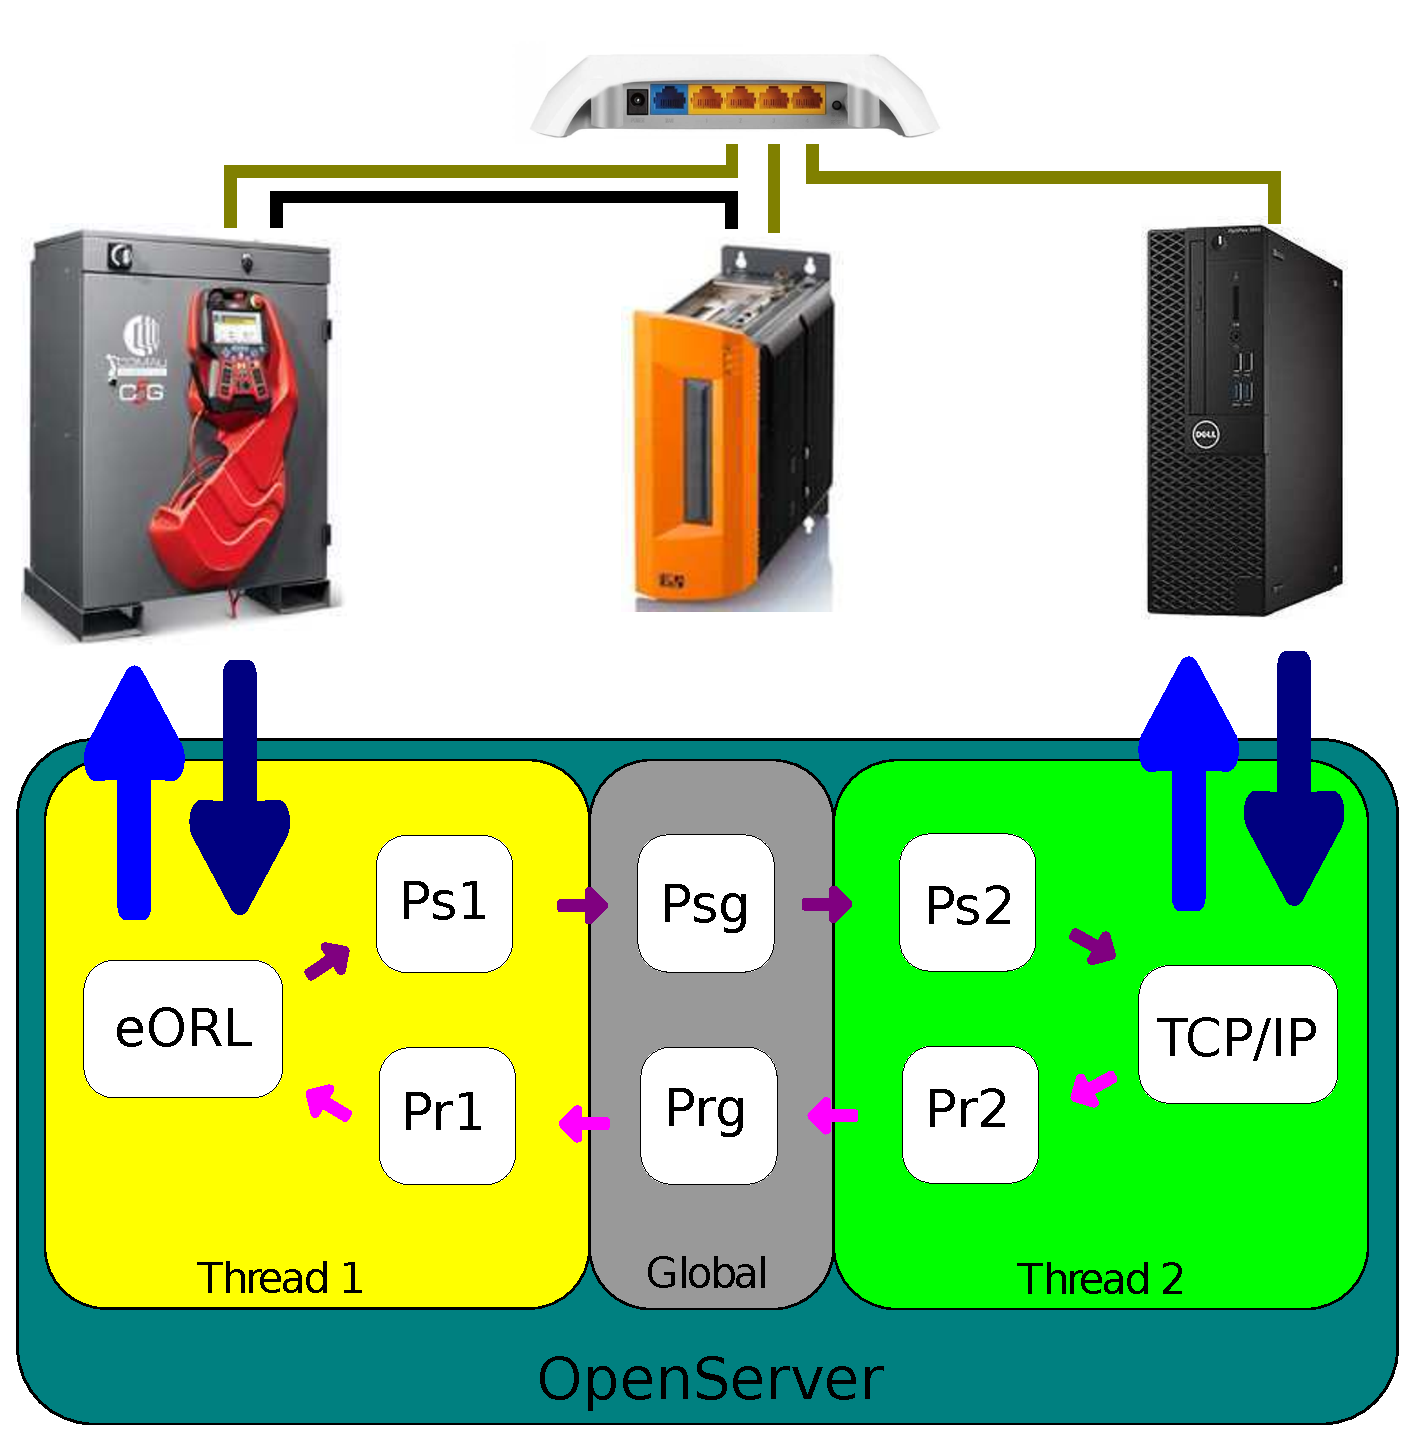
\includegraphics[width=10cm]{imagens/Softwares/ponteiro.eps}
                \small 
                \centering 
                \caption{Funcionamento dos ponteiros inteligentes no OpenServer}
                \label{fig:ponteiros}
            \end{figure}
        
            Desta forma, enquanto a thread de comunicação com o cliente não atualiza na variável global os valores de referência das juntas do robô, a thread de comunicação com a controladora envia repetidamente a última referência salva. Quando a thread de comunicação com o cliente for ler os dados sensoriais da junta do robô no ponteiro global, ela irá ler o pacote de dados mais recente, pois a thread de comunicação com a controladora está continuamente atualizando o pacote de dados em tal ponteiro.
            
            Essa abordagem soluciona o problema da assincronia de comunicação, pois quando ocorre a tentativa de atribuição de um objeto de um ponteiro inteligente local em um global em uma thread, ao mesmo tempo que acontece a tentativa de atribuição de uma ponteiro inteligente global em um local por outra thread, o ponteiro inteligente tem um mecanismo de gerenciamento para tal situação. Ele cria um segundo objeto para ser atribuído enquanto o primeiro é lido. Depois, o primeiro é automaticamente destruído e o segundo objeto passa a ocupar o lugar do primeiro.
        
    \section{O OpenClientExemple}
    
        Para testar o OpenSever foi preciso desenvolver um programa cliente que se comunique com ele via rede \ac{TCPIP}. Este programa foi chamado de \textit{OpenClientExemple}, isto é, um exemplo de cliente do OpenServer. Ele foi escrito em C++ usando bibliotecas padrão para sistemas operacionais baseados em Linux e permite o usuário enviar os ângulos de referência de cada junta do robô e visualizar as leituras dos sensores de posição angular (\textit{encoder} absoluto de precisão) de cada junta em tempo real através de uma interface gráfica que pode ser vista na Figura~\ref{openclient_}. 
    
        \begin{figure}[H]
            \centering
            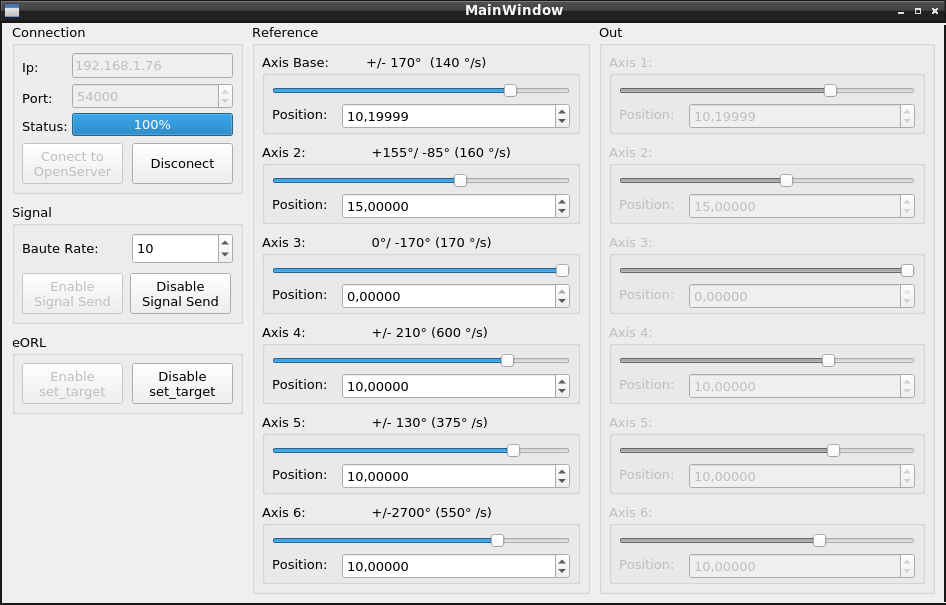
\includegraphics[width=\columnwidth]{imagens/Softwares/openclient_.png}
            \small 
            \centering 
            \caption{Interface gráfica do \textit{OpenClientExemple}}
            \label{openclient_}
        \end{figure}
        
        O funcionamento dele é simplesmente, depois de iniciar a conexão com o OpenServer, ler os valores dos componentes da interface gráfica e enviar para o OpenServer, ao mesmo tempo que recebe os ângulos das juntas vindos do OpenServer e os atualiza nos componentes da interface gráfica.
        
    \chapter{Resultados e discussões}
    \label{chp:Resultados}
    
    Antes de coletar os resultado, primeiramente o OpenServer foi compilado e executado no \ac{LPC} conectado à controladora do robô, o qual ficou aguardando conexão via rede \ac{TCPIP}, como esperado.
    
    Já o \textit{OpenClientExemple} foi compilado e executado em dois dispositivos diferentes, um \ac{PC} de arquitetura \textit{x86-64} e um \ac{SBC} de arquitetura \textit{arm64}. Durante a execução do OpenServer a taxa de amostragem foi aferida imprimindo no terminal o tempo que um pacote foi enviado e depois realizando a subtração do tempo atual pelo tempo do último pacote enviado. Os dados foram salvos em uma tabela e convertidos em gráficos.
    
    \section{Teste com PC \textit{x68-64}}
    
        O computador pessoal estava executando o sistema operacional Debian 11 de 64bits, com Kernel Linux Genérico e ambiente de desktop LXDE. É importante ressaltar o ambiente de desktop pois ele pode ser um dos principais responsáveis pelo consumo de processamento do computador, influenciando diretamente nos resultados dos testes. Por este motivo foi escolhido o LXDE, que é um dos ambientes de desktop com menos consumo de processamento que existe.
        
        As informações de hardware mais possivelmente impactantes nos resultados coletados estão listadas abaixo.
        \begin{enumerate}
            \item CPU: Intel Core i7 8550U
            \item GPU: Intel UHD Graphics 620
            \item Memória RAM: DDR4 - 16GB - Single Channel - 2400MHz
            \item Memória ROM: SSD NVME - 512GB - 1500MB/s
            \item Porta ethernet: Gigabit
        \end{enumerate}
        
        Apesar da porta de ethernet ser gigabit, o roteador utilizado só tinha capacidade para conexões de 100 megabits.
        
        Os resultados dos testes de taxa de amostragem do \ac{PC} podem ser vistos na Figura~\ref{fig:resultado_notebook}, onde o eixo horizontal representa cada amostra coletada e o eixo vertical o tempo em microssegundos.
        
        \begin{figure}[h]
            \centering
            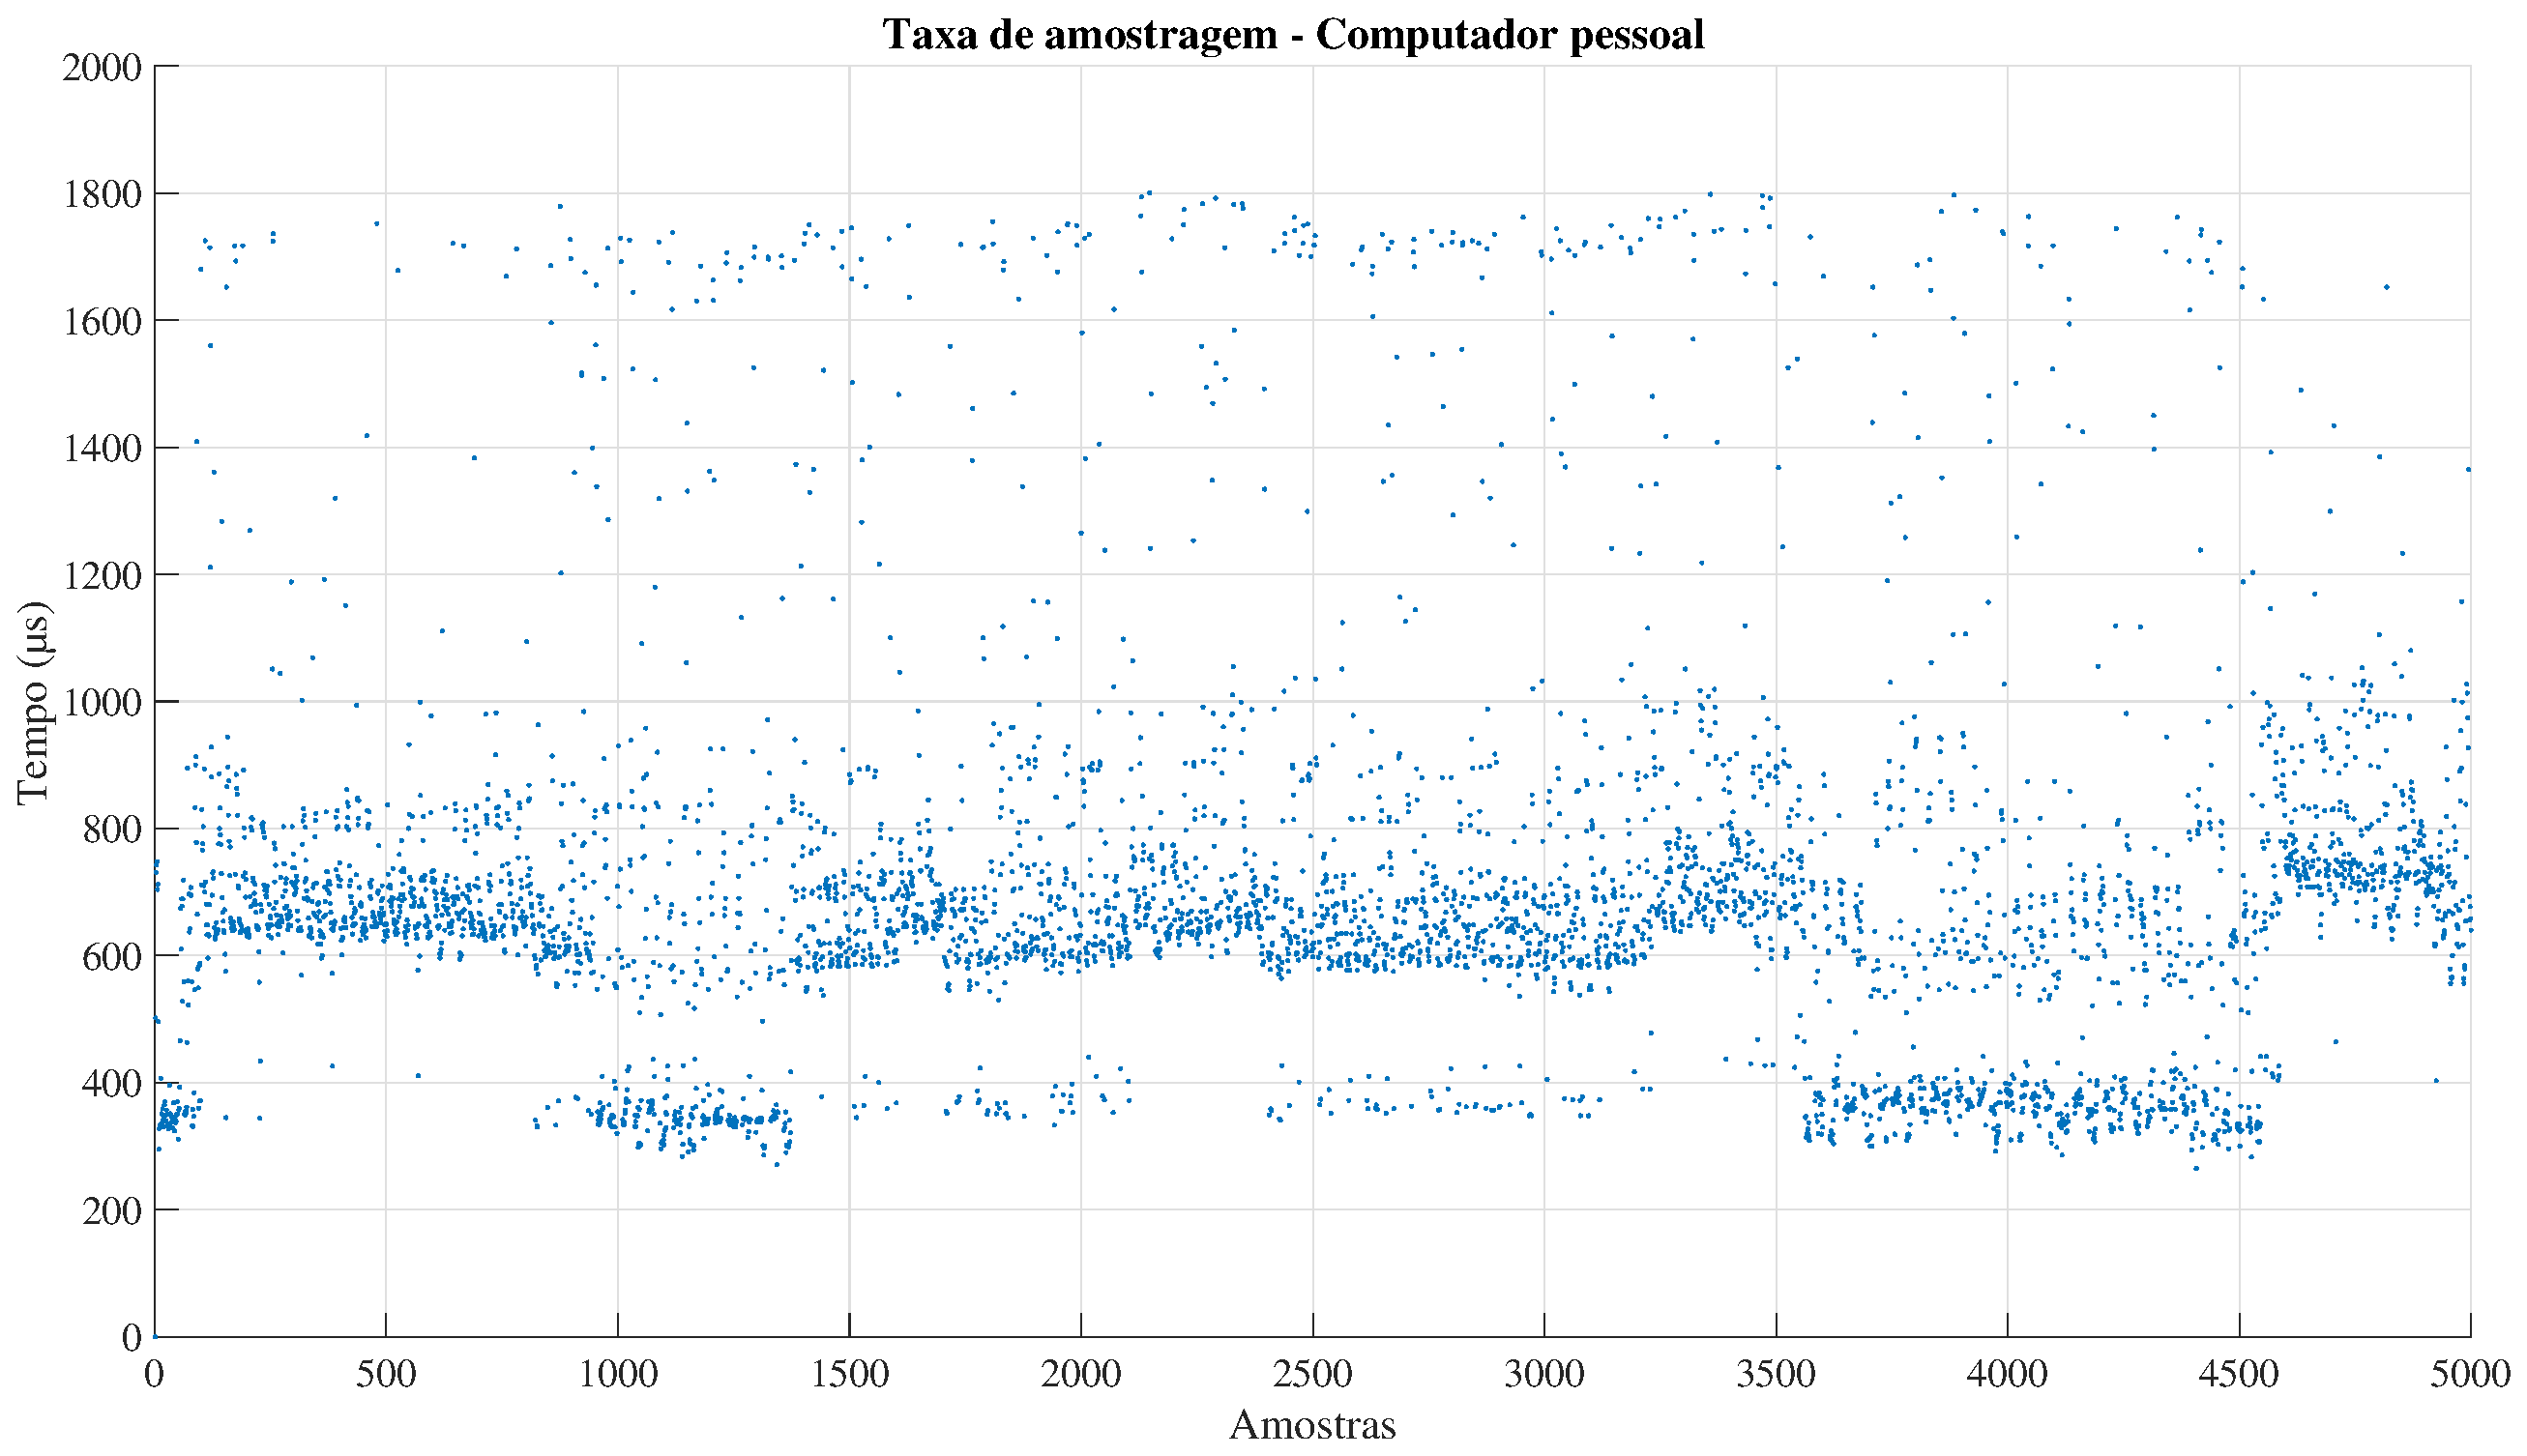
\includegraphics[width=\columnwidth]{imagens/Resultados/testeNote.eps}
            \small 
            \centering 
            \caption{Resultado Notebook}
            \label{fig:resultado_notebook}
        \end{figure}
    
    %single board computer
    \section{Teste com SBC \textit{arm64}}
        
        O \ac{SBC} utilizado nos testes foi o Raspberry Pi 4 Model B executando o sistema operacional Raspberry Pi OS Buster de 64 bits, que na verdade é o sistema operacional Debian 10 com algumas modificações desenvolvidas pela empresa Raspberry. O ambiente desktop é o LXDE-Pi, uma variante do LXDE desenvolvida para o sistema Raspberry Pi OS.
        
        As informações de hardware mais possivelmente impactantes nos resultados coletados estão listadas abaixo.
        \begin{enumerate}
            \item CPU: ARM Cortex A72 QuadCore - 1.5GHz
            \item GPU: Broadcom VideoCore VI - 500MHz
            \item Memória RAM: LPDDR4 - 8GB - Single Channel - 3200MHz
            \item Memória ROM: Cartão SD - 170MB/s
            \item Porta ethernet: Gigabit
        \end{enumerate}
        
        Apesar da porta de ethernet ser gigabit, foi utilizado o mesmo roteador do teste anterior que apenas tem a capacidade para conexões de 100 megabits.
        
        Os resultados dos testes de taxa de amostragem do \ac{SBC} podem ver vistos na Figura~\ref{fig:resultado_PI}, onde o eixo horizontal representa cada amostra coletada e o eixo vertical o tempo em micro segundos.
        
        \begin{figure}[h]
            \centering
            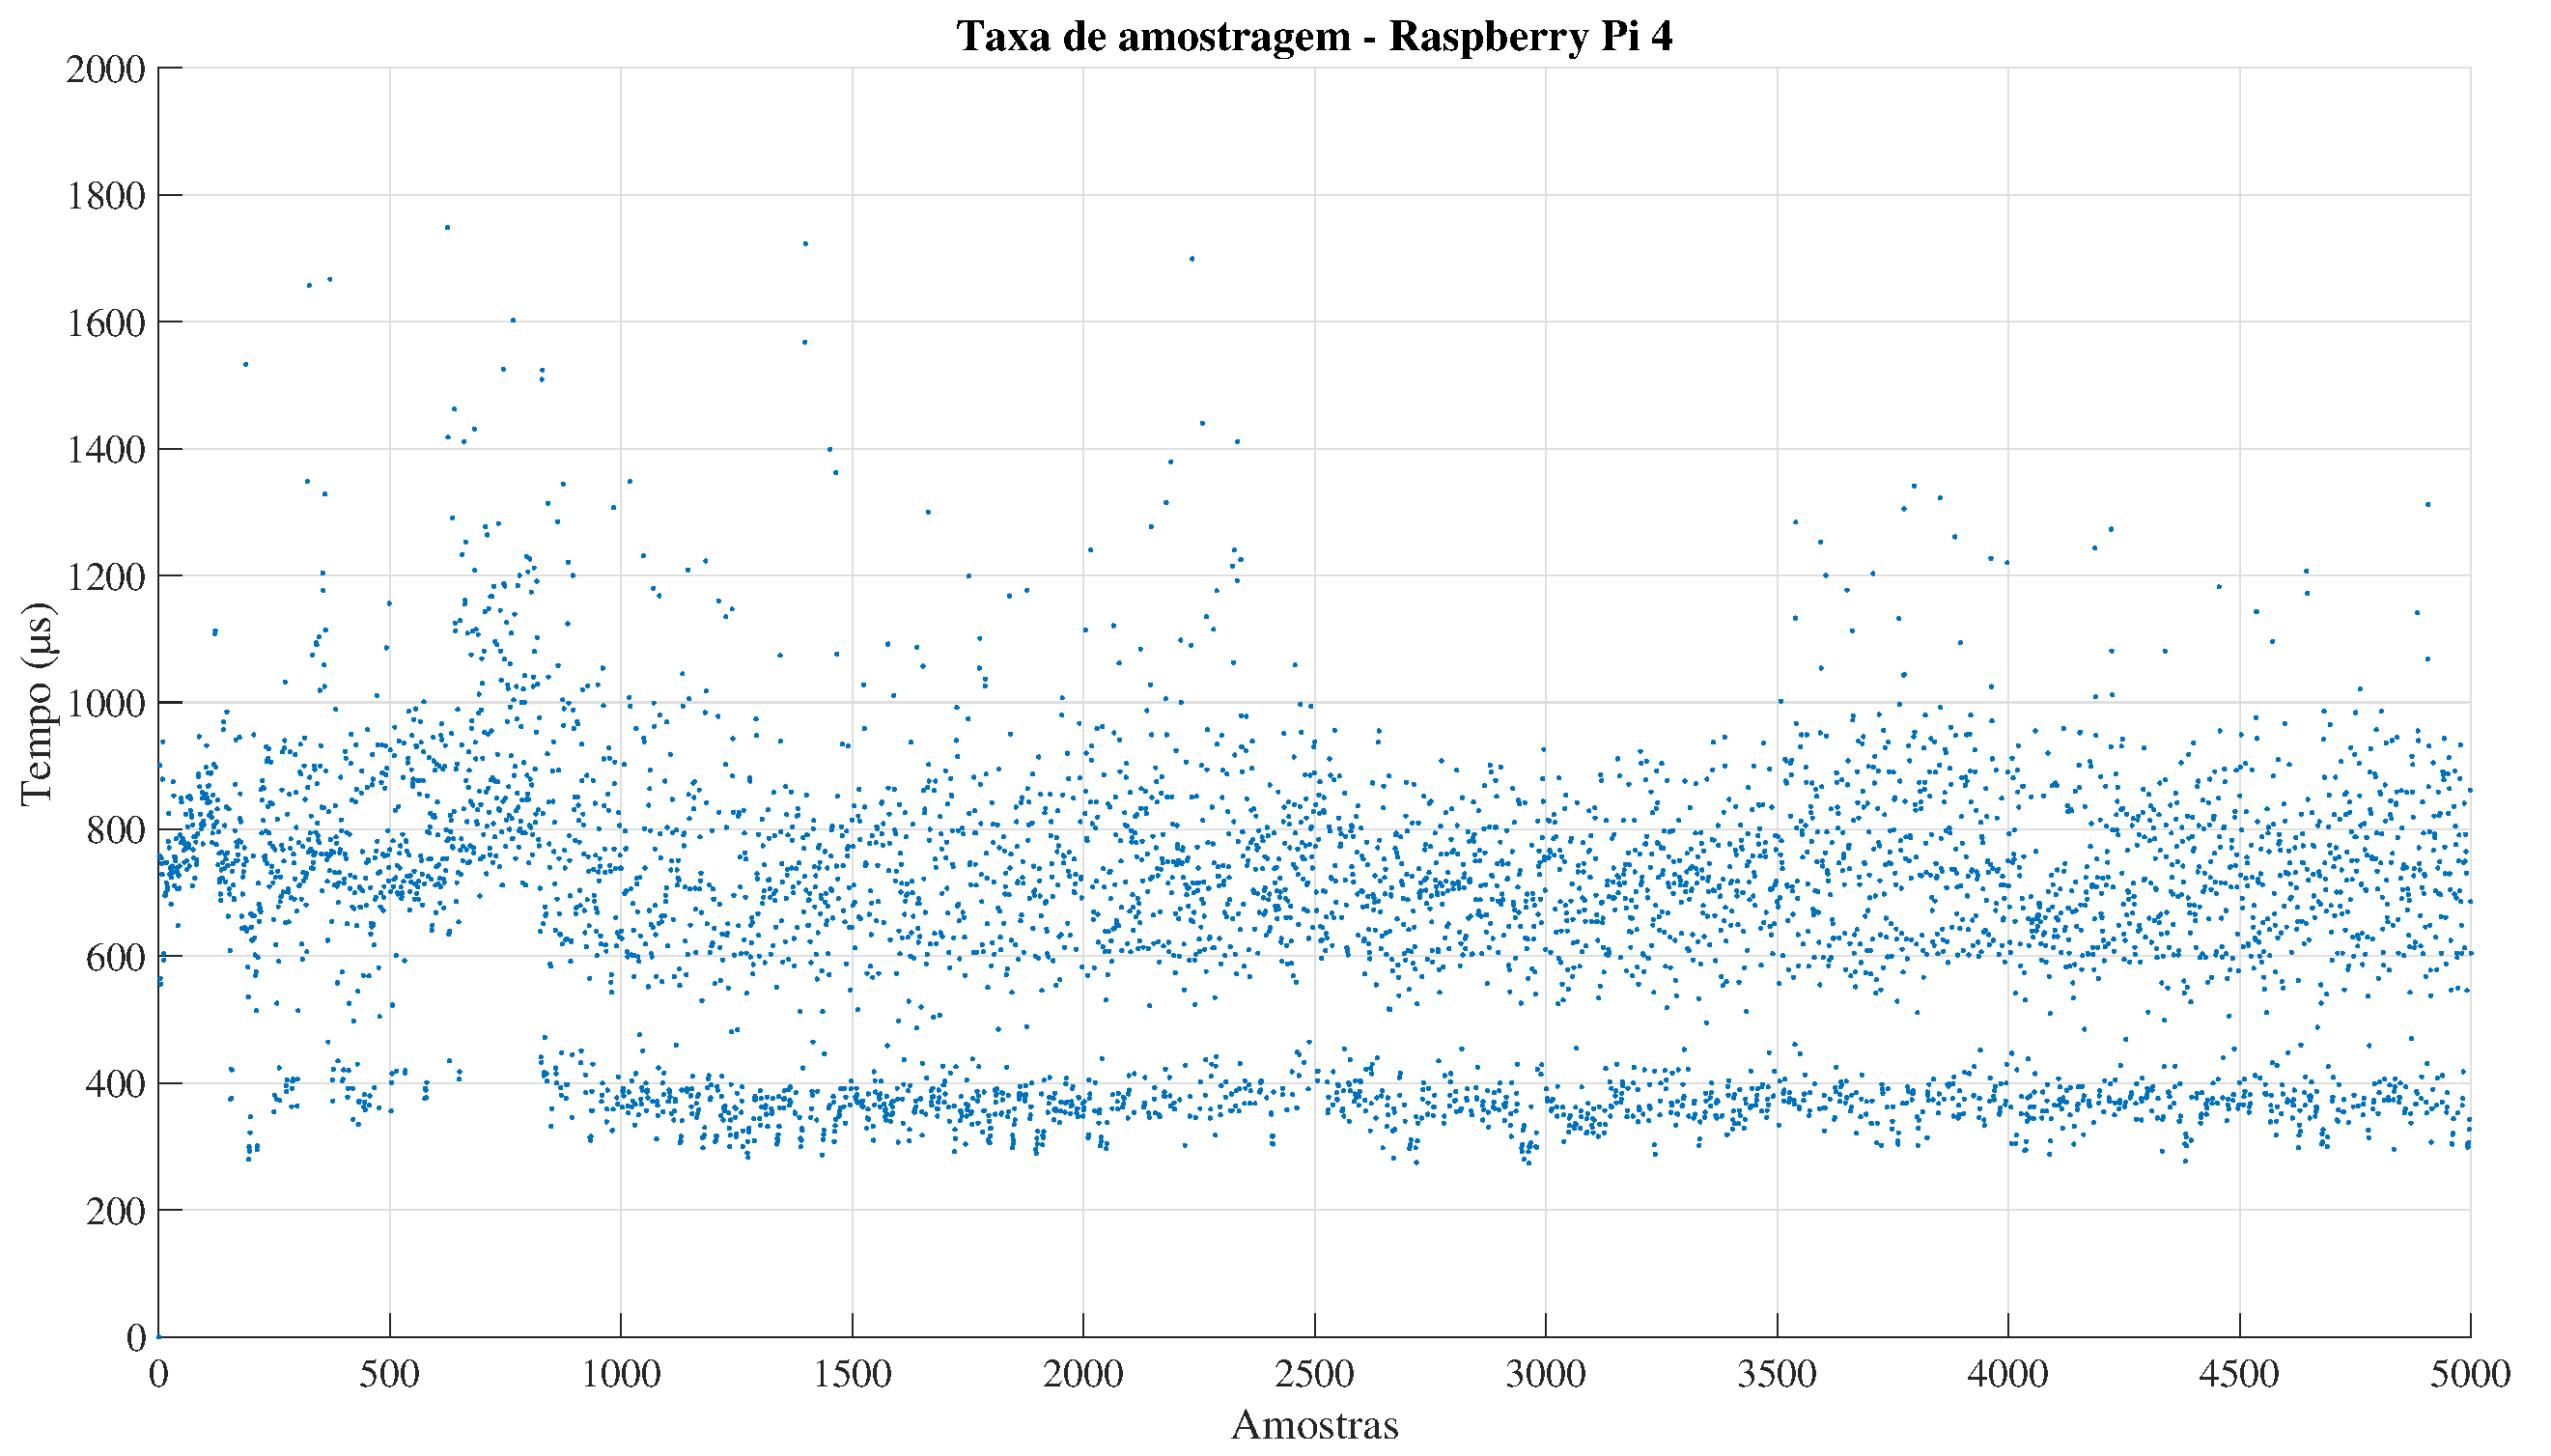
\includegraphics[width=\columnwidth]{imagens/Resultados/testePi.eps}
            \small 
            \centering 
            \caption{Resultado PI}
            \label{fig:resultado_PI}
        \end{figure}
        
    \section{Teste de conexão com outras linguagens, dispositivos e sistemas operacionais}
    
       A fim de verificar se é possível estabelecer a conexão com o OpenServer utilizando outras linguagens de programação e dispositivos foram testadas a linguagem Python e MatLab. A conexão foi estabelecida com sucesso usando a biblioteca padrão \ac{TCPIP} dos mesmos, demonstrando que é possível desenvolver programas clientes em linguagens de programação diferentes da linguagem da biblioteca \ac{eORL}. Como ambos testes foram realizados utilizando o Sistema Operacional \textit{Windows}, foi demonstrando também que podem ser desenvolvidos softwares para outros sistemas operacionais.
       
       Foi testada a comunicação com um dispositivo móvel rodando o sistema operacional \textit{Android} através de um aplicativo genérico de conexão \ac{TCPIP}. O dispositivo móvel estava conectado à rede interna através de conexão sem fio. A comunicação foi bem sucedida, demonstrando que podem ser desenvolvidos softwares clientes para \textit{smartphones} controlarem o braço robótico através do OpenServer e demonstrando também que a rede sem fio pode ser utilizada para conexão com o mesmo.
    
    \section{Discussões}
        
        Em ambos os testes nenhum pacote foi enviado a uma taxa maior que \SI{1800}{\micro\second}, logo é possível estabelecer que \SI{2}{\milli\second} é a menor taxa estável, considerando uma margem de segurança, para os hardwares testados. Apesar de provavelmente essa taxa ser suficiente para atender a maioria das aplicações, acredita-se que ela possa ser melhorada desenvolvendo-se outros protocolos \ac{TCPIP} para transmitir os dados, por exemplo, transmitindo diretamente os valores binários das memórias ao invés de converter em um pacote de strings.
        
        Analisando ambos gráficos, é possível perceber que no computador pessoal ocorreu uma quantidade maior de amostras em torno de \SI{1800}{\micro\second}, logo é possível afirmar que a taxa de amostragem do Raspberry Pi 4 foi mais estável. Provavelmente esse fato se dá que a frequência da memória RAM do Raspberry Pi 4 utilizado é superior, cerca de $30\%$ a mais.
        
        O \textit{OpenClientExemple} foi um programa desenvolvido com o objetivo de testar o interpretador de comandos OpenServer e poder movimentar o robô através do mesmo, logo ele possui uma interface gráfica onde o usuário pode alterar as referências de cada junta, assim testando se o OpenServer está interpretando corretamente as referências enviadas pelo protocolo. Em uma thread separada, os dados da interface gráfica são enviados pelo protocolo TCP/IP e o tempo de envio é imprimido no terminal. Talvez essa abordagem não tenha sido favorável a coletar resultados de taxa de amostragem pois a interface gráfica pode estar consumindo processamento e aumentando a taxa de amostragem, ou talvez a biblioteca de tempo utilizada para executar a thread não seja tão precisa quanto necessário para estes teste.
        
        Para realização de testes mais precisos seria necessário alterar a código do exemplo a fim de retirar a interface gráfica e enviar em loop os pacotes via \ac{TCPIP} pela thread principal, assim dispensando a biblioteca que executa a thread com base no relógio do sistema.
        
        Com base nisso é possível afirmar que a taxa máxima tem que ser analisada para cada dispositivo que vai ser executado o programa cliente e que o OpenServer cumpriu o seu papel de permitir realizar uma taxa de comunicação diferente da controladora e inclusive em taxas não constantes.
    \chapter{Conclusão}
    \label{chp:Conclusão}

    %Justificativa -> tema
    Este trabalho de pesquisa foi iniciado diante da necessidade de se investigar se seria possível dar mais liberdade no desenvolvimento de aplicações para um robô industrial com controladora aberta, atendendo inclusive a demanda do Laboratório de Robótica do CEFET-MG.
    
    %Objetivo Geral (se foi atendido)
    Diante disso, o objetivo geral do trabalho foi desenvolver um software com um arranjo cliente servidor que estenda a liberdade que a solução da fabricante proporciona aos programadores de robôs industriais. Tal software foi desenvolvido e o objetivo geral foi atingido.
    
    %Cada um dos objetivos Específicos (se foi atingido)
    O protocolo de comunicação TCP/IP para enviar e receber variáveis referentes aos ângulos de juntas do robô foi criado, permitindo que softwares clientes programados nas mais diversas linguagens de programação e sistemas operacionais se comuniquem fazendo uso dele, atingindo assim o primeiro objetivo específico.
    
    A função que comunica com a controladora do robô, salvando e enviando informações da memória, foi implementada, bem como a função que se comunica com o software cliente, salvando e enviando informações da memória, atingindo assim o segundo e o terceiro objetivos específicos.

    E por fim, o problema gerado pelo assincronismo da comunicação do OpenServer com a controladora e o programa cliente foi solucionado através do uso de ponteiros inteligentes para salvar as informações na memória, garantindo assim que não ocorra problemas na atribuição de valores na memória no momento da leitura dos mesmos. Assim, o último objetivo específico foi atingido.
        
    %Relato das descobertas dos objetivos específicos
    %Foi descoberto que 
    
    %Hipótese (Qual foi? Confirmada ou refutada)
    Partiu-se da hipótese que é possível desenvolver um software que se comunique ao mesmo tempo com a controladora do robô e com um programa cliente, porém em taxas diferentes, sendo este dispositivo de outra arquitetura e o software programado em uma linguagem diferente e rodando em um sistema operacional diferente. A hipótese foi confirmada e tal software desenvolvido.
    
    %Limitações: Dificuldades encontradas - Limitações da pesquisa
    Uma limitação atual da pesquisa está sendo diagnosticar o gargalo do sistema que impede a comunicação de ocorrer a uma taxa menor que \SI{2}{\milli\second} de forma estável.
    
    %Recomendações: Consequência das dificuldades, recomendar continuidade
    Uma forma de superar esse gargalo seria desenvolver um programa cliente mais simples específico para coleta de dados de taxa de amostragem e implementar um protocolo adicional de comunicação que envie informações direto da memória RAM sem os converter em \textit{strings}, como foi feito nesse trabalho
    
    \section{Perspectivas futuras}
        
        Com objetivo de atingir taxas de comunicação maiores, está em fase de estudos o desenvolvimento de protocolos de comunicação mais otimizados com base em \ac{TCPIP}. Por exemplo, criando uma nova modalidade, desta vez de forma síncrona, que envie dados ao mesmo tempo que recebe, ao invés de usar a forma assíncrona, que aguarda o recebimento de um dado para enviar o próximo. Espera-se que isso dobre a taxa de comunicação.
        
        Outra modalidade em fase de estudos seria, como já citado, transmitir os dados binários direto da memória RAM. Essa modalidade talvez seja menos compatível com outras linguagens de programação, mas é focada em aplicações com a necessidade específica de taxas de amostragens mais altas. 
        
        Está sendo elaborado o desenvolvimento um programa cliente do OpenSever que adiciona ao sistema robótico uma malha de controle baseada em visão computacional. Uma câmera afixada no efetuador do robô filma uma figura de referência, o software cliente processa a imagem e gera as referências que são enviados ao OpenServer, de forma a manter constante a pose (posição e orientação) do manipulador robótico em relação à pose da figura de referência. Dessa maneira, é adicionada uma câmera à estrutura desenvolvida, conforme é representado na Figura~\ref{pespectiva}, onde (1) representa a câmera e (2) a figura de referência.
    
        \begin{figure}[ht]
            \centering
            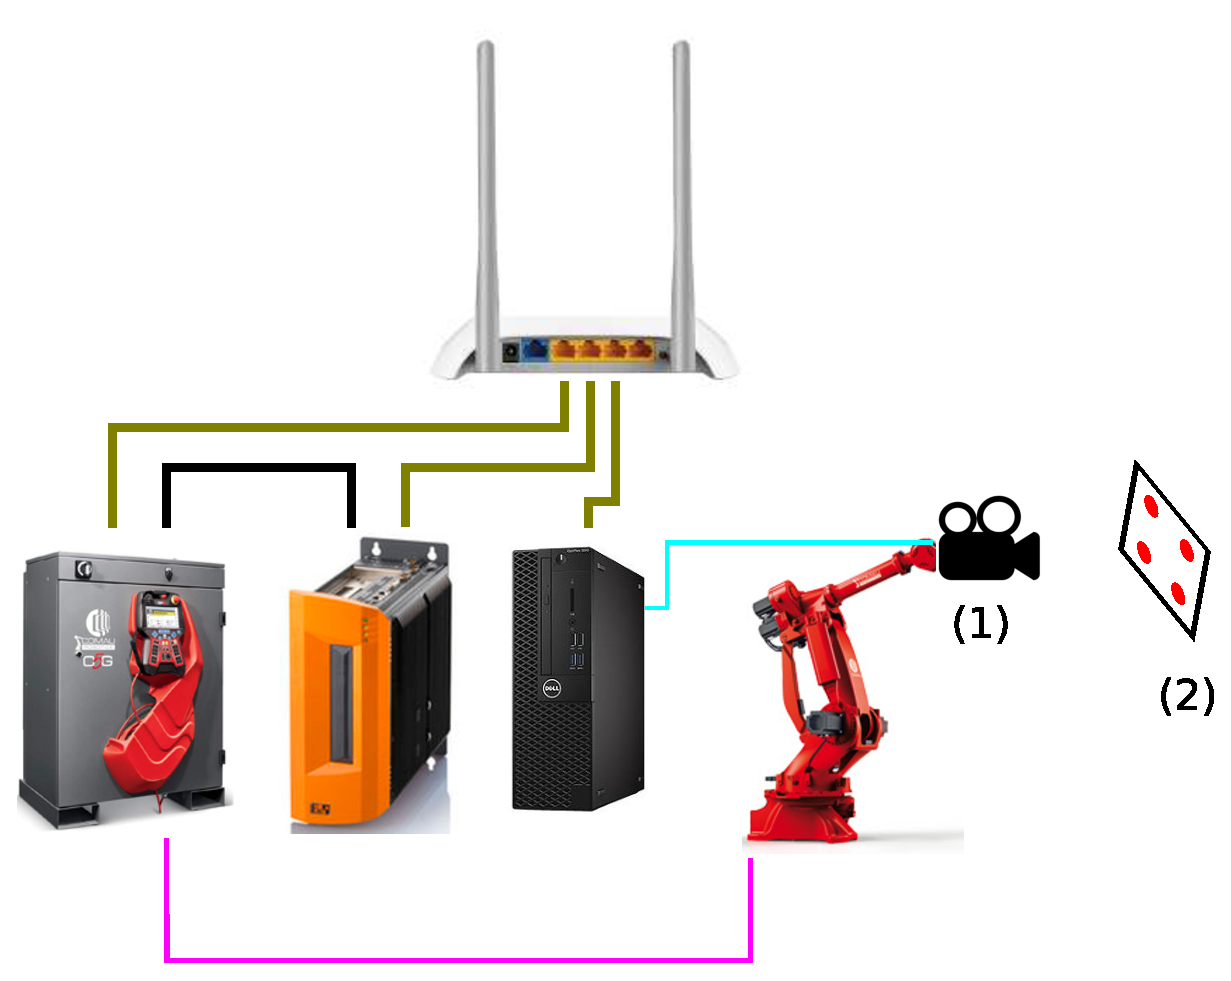
\includegraphics[width=\columnwidth]{imagens/pespectiva.eps}
            \small 
            \centering 
            \caption{Estrutura proposta para utilização do OpenServer}
            \label{pespectiva}
        \end{figure}        

    \printbibliography{}
\end{document}
